\documentclass[conference,a4paper]{IEEEtran}

% ---------------------------------------------------------------
% Packages
% ---------------------------------------------------------------
\usepackage[T1]{fontenc}
\usepackage[utf8]{inputenc}
\usepackage{graphicx}
\usepackage{booktabs}
\usepackage{tabularx}
\usepackage{array}
\usepackage{makecell}
\usepackage{amsmath}
\usepackage{xcolor}
\usepackage{microtype}
\usepackage[hidelinks]{hyperref}
\usepackage{url}
\def\UrlBreaks{\do\/\do\_\do\.}
\urlstyle{tt}

\newcolumntype{L}{>{\raggedright\arraybackslash}X}
\newcolumntype{P}[1]{>{\raggedright\arraybackslash}p{#1}}
\newcommand{\var}[1]{\texttt{#1}}
\newcommand{\tabnote}[1]{\par\vspace{3pt}\begin{minipage}{\linewidth}\footnotesize\raggedright #1\end{minipage}}
\graphicspath{{figures/}{../figures/}}
\renewcommand{\arraystretch}{1.12}
\setlength{\emergencystretch}{3em}
\renewcommand{\topfraction}{0.9}
\renewcommand{\bottomfraction}{0.8}
\renewcommand{\textfraction}{0.07}
\renewcommand{\floatpagefraction}{0.6}
\renewcommand{\dbltopfraction}{0.9}
\renewcommand{\dblfloatpagefraction}{0.5}
\setcounter{topnumber}{3}
\setcounter{bottomnumber}{3}
\setcounter{totalnumber}{5}
\setcounter{dbltopnumber}{3}
\sloppy
\raggedbottom

\begin{document}

\title{ElimuSentry - Phase 2: Building the Preprocessing Pipeline\\
\large What was built, what the diagnostics showed, and where reality changed the plan}

\author{\IEEEauthorblockN{Emile Lucky Muhigira}
\IEEEauthorblockA{Carnegie Mellon University Africa, Kigali, Rwanda\\
emuhigir@andrew.cmu.edu\\
04-652 Artificial Intelligence System Design, Assignment 2, Phase 2 (Strategy Execution, Pipeline and Visual Diagnostics)\\
Repository: \url{https://github.com/Emile-Lucky-Muhigira/AISD_Project}}}

\maketitle

\begin{abstract}
Phase 1 planned, with evidence, how every piece of information about a child in the Ghana Socioeconomic Panel Survey would be prepared for a school-dropout early-warning model. This report covers Phase 2: turning that plan into working code and checking it. The plan was built as one scikit-learn \var{Pipeline} around a \var{ColumnTransformer}, with seven custom steps in \path{src/transformers.py}. It is fitted on the model-building children only (X\_train, 1,307 children from 2009/10) and then applied unchanged to the testing children (X\_test, 1,395 children from 2013/14). The output has exactly the planned size: 33 features become 30, and then 53 numeric columns for XGBoost or 48 for logistic regression, with no missing value left. The three removed features can be rebuilt exactly from the kept ones (0 differences in 3,807 checks), so nothing is lost. Eight diagnostic figures confirm each step. Most decisions were carried out as planned; five points changed or were sharpened by what the data showed. Inflation explains only about half of the rise in household-goods value between visits. The choice of which feature to drop in a repeating pair is not stable from fold to fold, so the tie-break rule decides. The hours-missed rule makes no measurable difference against a median fill. The ``was missing'' flags are switched on about half as often in the later period. And rank correlation was needed because the ordinary correlation would have missed one repeating pair.
\end{abstract}

\begin{IEEEkeywords}
data preprocessing, scikit-learn pipeline, leakage prevention, visual diagnostics, school dropout, Ghana panel survey
\end{IEEEkeywords}

% ===============================================================
\section{Introduction}
% ===============================================================
\textbf{Aim of this phase.} Phase 1 used the Ghana Socioeconomic Panel Survey \cite{gsps} and decided how to fill gaps, treat extreme values, remove repeating features, encode categories, rescale numbers and split the data without leakage \cite{phase1}. Phase 2 has three tasks, which follow the assignment: (1) implement that strategy as fully runnable code with a strict X\_train / X\_test separation; (2) check every assumption with eight diagnostic figures; and (3) record where reality agreed with the plan and where it forced a change.

\textbf{What is in the repository.} \path{src/transformers.py} holds the custom preparation steps; \path{src/pipeline_builder.py} assembles them into the pipeline; \path{phase2_implementation/notebooks/pipeline_execution.ipynb} runs everything from start to finish, saves the eight figures to \path{figures/} at 300 DPI, writes the processed tables to \path{data/processed/} and the decision log to \path{phase2_implementation/decision_log.csv}. The notebook was run from top to bottom without errors.

\textbf{Scope.} Phase 2 is about preparing the data. A quick five-fold run of two models is included only to prove that the full pipeline (preparation plus model) works end to end without leakage. Tuning the models, adjusting the risk percentages (calibration) and the single final test belong to the modelling phase, so the outcomes of the testing children are not used anywhere in this phase.

\textbf{Reading this report.} Technical terms are explained in plain language in the Appendix. Section~II describes what was built, Section~III the figures, Section~IV the decision log, Section~V the changes and their reasons, and Section~VI the checks on the output.

% ===============================================================
\section{What Was Built}
% ===============================================================
\begin{table*}[!t]
\centering
\caption{The pipeline, step by step, in the order the data pass through it}
\label{tab:steps}
\footnotesize
\setlength{\tabcolsep}{4pt}
\renewcommand{\arraystretch}{1.0}
\begin{tabularx}{\textwidth}{c P{3.4cm} L P{3.2cm} c}
\toprule
\# & Step (code name) & What it does & Learns from & Phase 1 \\
\midrule
0 & \path{deflate_to_2009_prices} & Divides 2013/14 money amounts by 1.62 to express them in 2009/10 prices & Nothing (fixed number) & C1 \\
1 & \var{MissedHoursRule} & A blank ``hours missed'' becomes 0 when attendance was recorded & Nothing (fixed rule) & B1 \\
2 & \var{MissingFlagger} & Adds the four yes/no ``was missing'' flags before any gap is filled & Nothing (fixed rule) & B1 \\
3 & \var{GradeKNNImputer} & Fills a missing school grade from the 5 most similar children, then recalculates years over-age & X\_train (neighbours) & B1 \\
4 & \var{ColumnDropper} & Removes people per room, lost a parent and school grade (33 $\rightarrow$ 30) & Nothing (fixed list) & B4b \\
5 & \var{CategoryRecoder} & Turns 1/2 answers into 0/1, reverses the textbooks scale, groups relationship to head into 3 options & Nothing (fixed rule) & C1 \\
6 & \var{SimpleImputer} (in the \var{ColumnTransformer}) & Fills gaps: average for balanced numbers, middle value for lopsided ones, most common answer for yes/no and ordered items, a ``missing'' option for school type & X\_train (averages, middle values, most common answers) & B1 \\
7 & \var{LogIQRCapper} & Caps travel time, household size and rooms at the IQR limit on the log scale; adds the log for the simple model & X\_train (limits) & B2, B3 \\
8 & \var{TrainingRank} & Turns the two money amounts into a 0--1 rank against the model-building children & X\_train (reference values) & C1 \\
9 & \var{OneHotEncoder} & One yes/no column per option of each label & X\_train (list of options) & C1 \\
10 & \var{StandardScaler} (simple model only) & Puts every number on a common scale (average 0, spread 1) & X\_train (average, spread) & C1 \\
\bottomrule
\end{tabularx}
\tabnote{Steps 1--5 run one after another on the whole table because each one needs the result of the one before (for example, flags must be added before gaps are filled). Steps 6--10 run side by side on different groups of columns inside the \var{ColumnTransformer}. Step 0 is applied to X\_test before the pipeline. Code: \path{src/transformers.py} and \path{src/pipeline_builder.py}.}
\end{table*}

\textbf{One pipeline, two versions.} The pipeline is built with scikit-learn \cite{sklearn}. The same steps produce two versions of the data (Table~\ref{tab:steps}). The \textbf{XGBoost version} \cite{xgboost} keeps numbers in their own units, because a decision tree only compares values; it has 53 columns. The \textbf{logistic regression and PCA version} adds the log on long-tailed features and standardises every number, and leaves out one option per label as the reference; it has 48 columns. This follows Phase 1, C1 exactly.

\textbf{How leakage is prevented.} Every step that learns something (averages, middle values, neighbours, cap limits, money ranks, the list of options, the scaler) is inside the pipeline. The pipeline is \emph{fitted} on X\_train only and then only \emph{applied} to X\_test. Inside cross-validation it is fitted again on the building part of each fold. The notebook checks this directly: it saves the fitted pipeline, applies it to X\_test, and confirms that nothing it learned has changed \cite{kaufman2012}. The only step applied outside the pipeline, the inflation adjustment, uses a fixed published number, not the data.

\textbf{The split.} The split is by time, as planned: X\_train holds the 1,307 children first seen in 2009/10 (14.4\% dropped out) and X\_test the 1,395 children first seen in 2013/14 (10.4\%). The 220 children who appear in both tables are marked, so the main test result can exclude them (1,175 children). Within X\_train, five folds are formed by whole districts with the same dropout share (\path{StratifiedGroupKFold}); no district or household appears on both sides of any fold.

\textbf{The inflation factor.} Phase 1 promised to convert 2013/14 money to 2009/10 prices using Ghana's consumer price index. The interview dates in the raw survey files show that the first visit took place from November 2009 to April 2010 and the second, labelled 2013/14, mostly from March to October 2014, with a few households in 2015. Using World Bank annual consumer price inflation for Ghana \cite{wbcpi} (index 2009 = 100: 2010 = 110.7, 2014 = 172.6, 2015 = 202.3), weighted by the number of interviews in each year, the price level was 107.5 at the first visit and 174.0 at the second. Every 2013/14 amount is therefore divided by $174.0/107.5 = 1.62$.

% ===============================================================
\section{Visual Diagnostics}
% ===============================================================
\begin{figure*}[!t]
\renewcommand{\thefigure}{1.1}
\centering
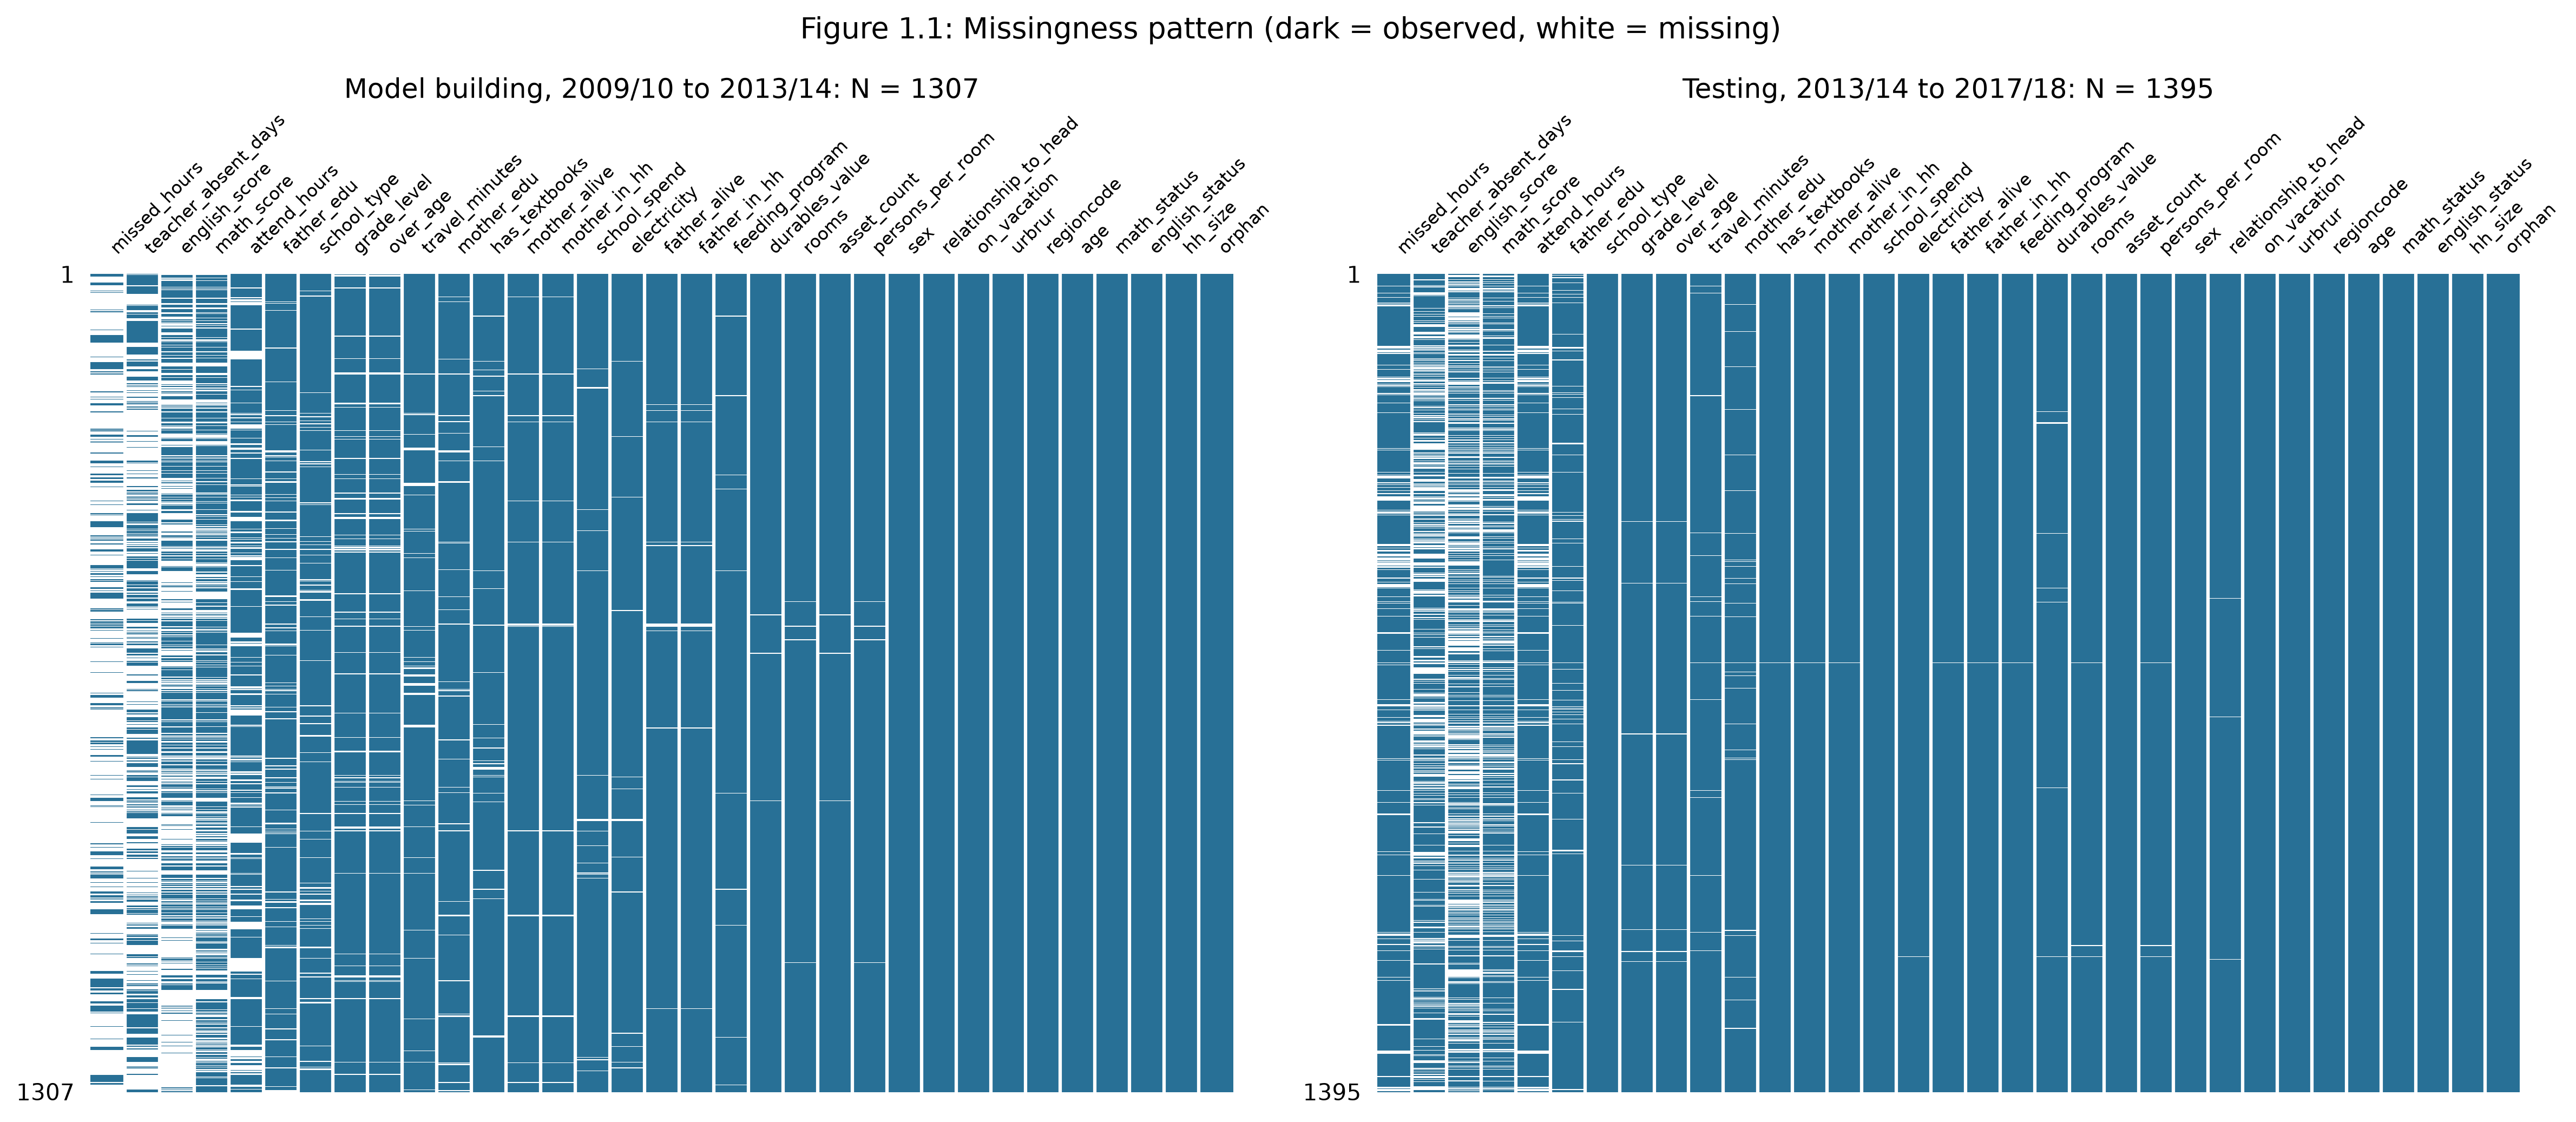
\includegraphics[width=0.78\textwidth]{fig1_1_missingness_heatmap.png}
\caption{Where answers are missing. Left: X\_train; right: X\_test. \emph{How to read it:} each thin row is one child and each column one feature; white marks are missing answers. The large white blocks on the left of X\_train are hours missed, days teacher absent, the two test scores and hours attended. X\_test has far fewer gaps because the 2013/14 tablets required an answer.}
\label{fig:missing}
\end{figure*}

\begin{figure}[!t]
\renewcommand{\thefigure}{1.2}
\centering
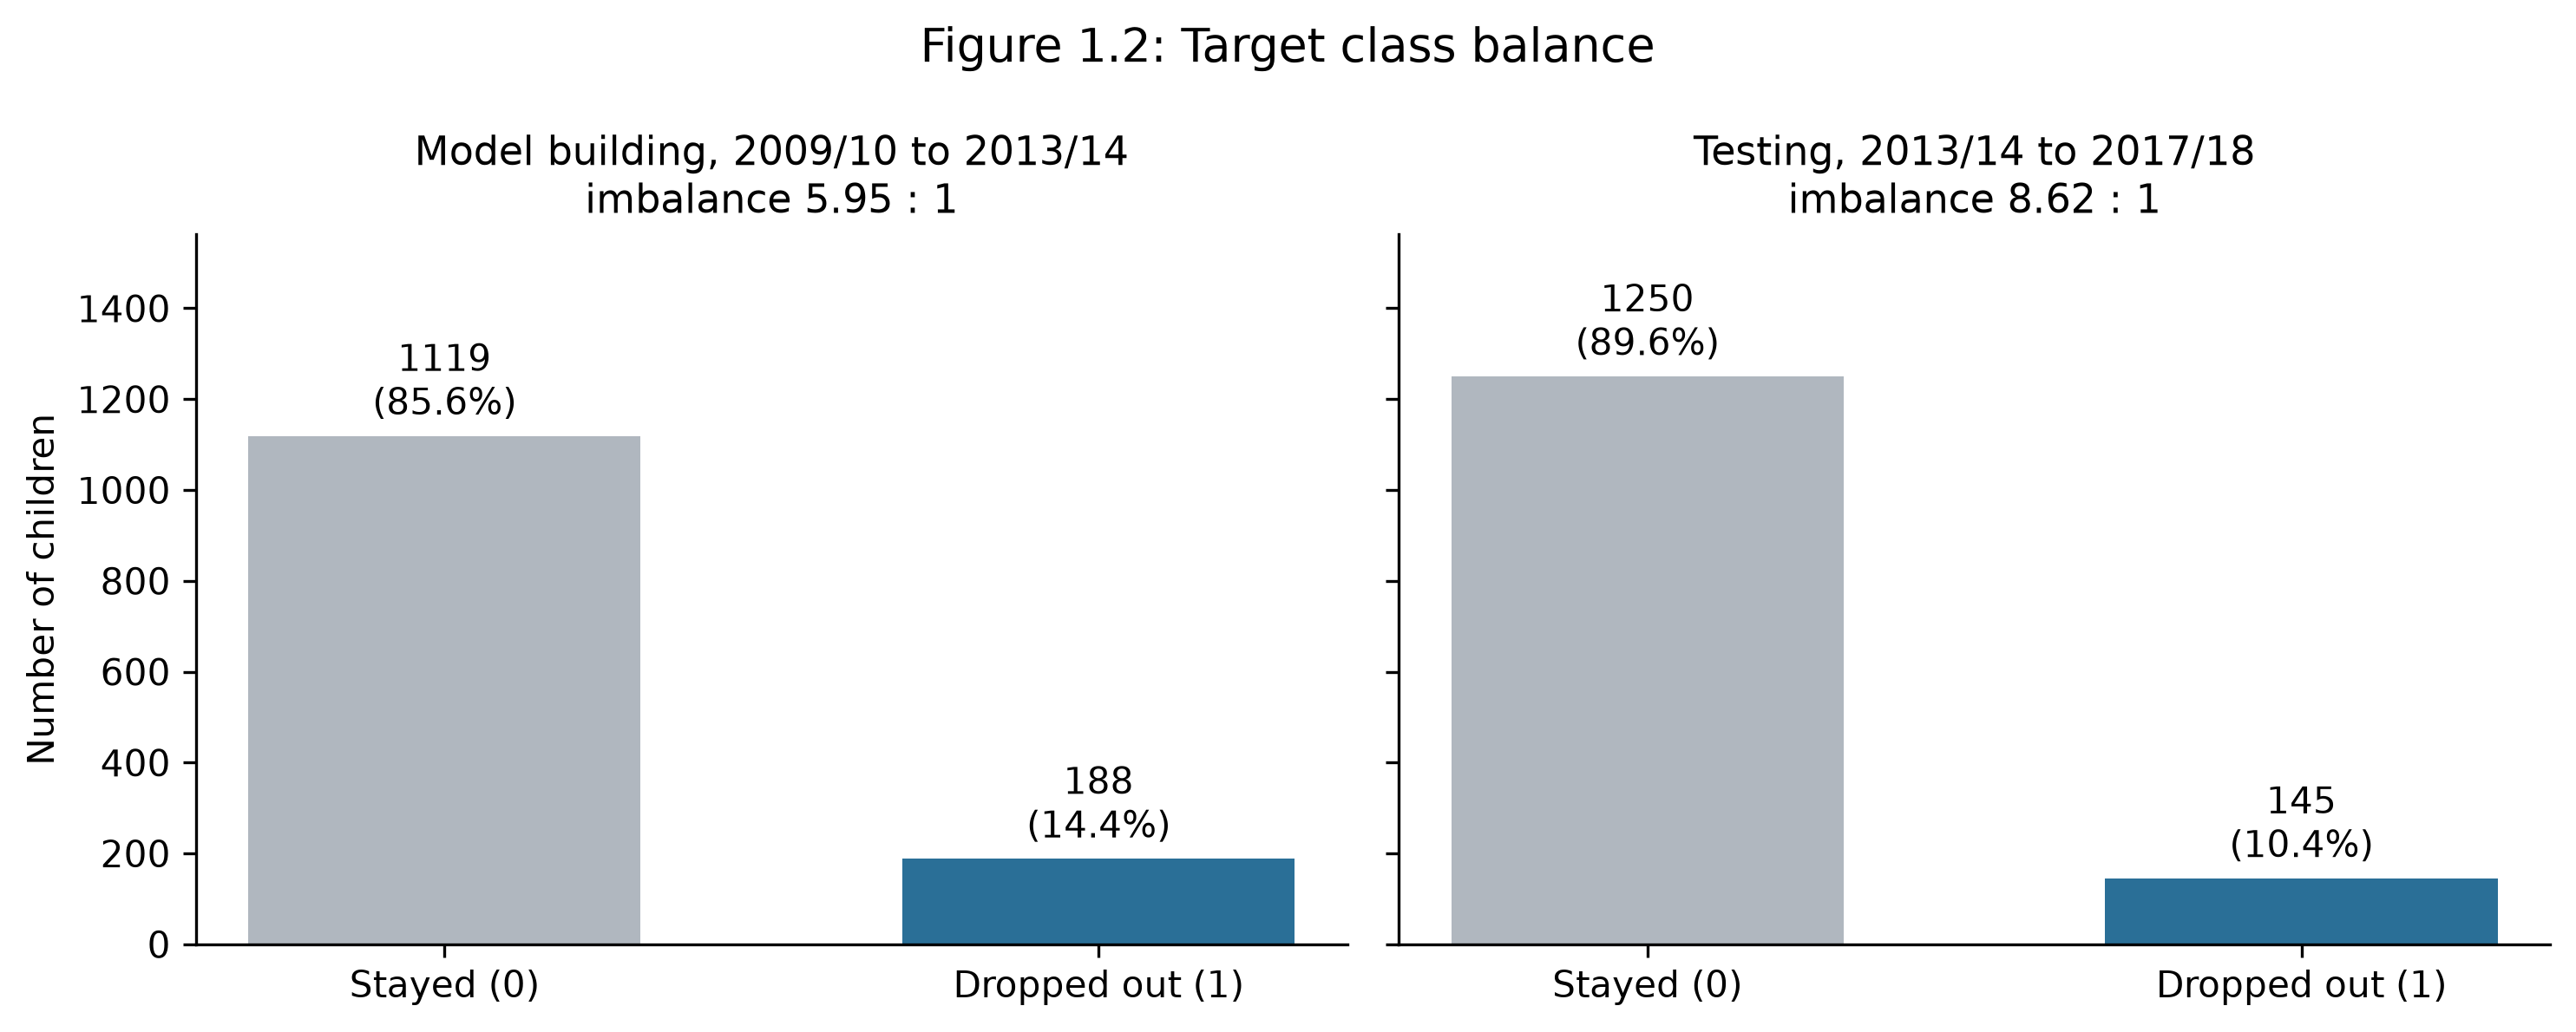
\includegraphics[width=\columnwidth]{fig1_2_target_distribution.png}
\caption{Children who stayed in school and who dropped out. X\_train: 188 of 1,307 dropped out (14.4\%, imbalance 5.95 : 1); X\_test: 145 of 1,395 (10.4\%, 8.62 : 1).}
\label{fig:target}
\end{figure}

\textbf{Missing answers (Fig.~\ref{fig:missing}).} The pipeline sees the same pattern as Phase 1: 3,820 of 43,131 answers missing in X\_train (8.86\%) and 1,826 of 46,035 in X\_test (3.97\%); 53 complete children in X\_train and 467 in X\_test. After the pipeline, \textbf{no missing value is left} in either table.

\textbf{Outcome (Fig.~\ref{fig:target}).} Dropouts are the small group in both periods, so each dropout is given extra weight during training (\var{scale\_pos\_weight} for XGBoost, \path{class_weight="balanced"} for logistic regression), recalculated inside every fold.

\begin{figure*}[p]
\renewcommand{\thefigure}{2.1}
\centering
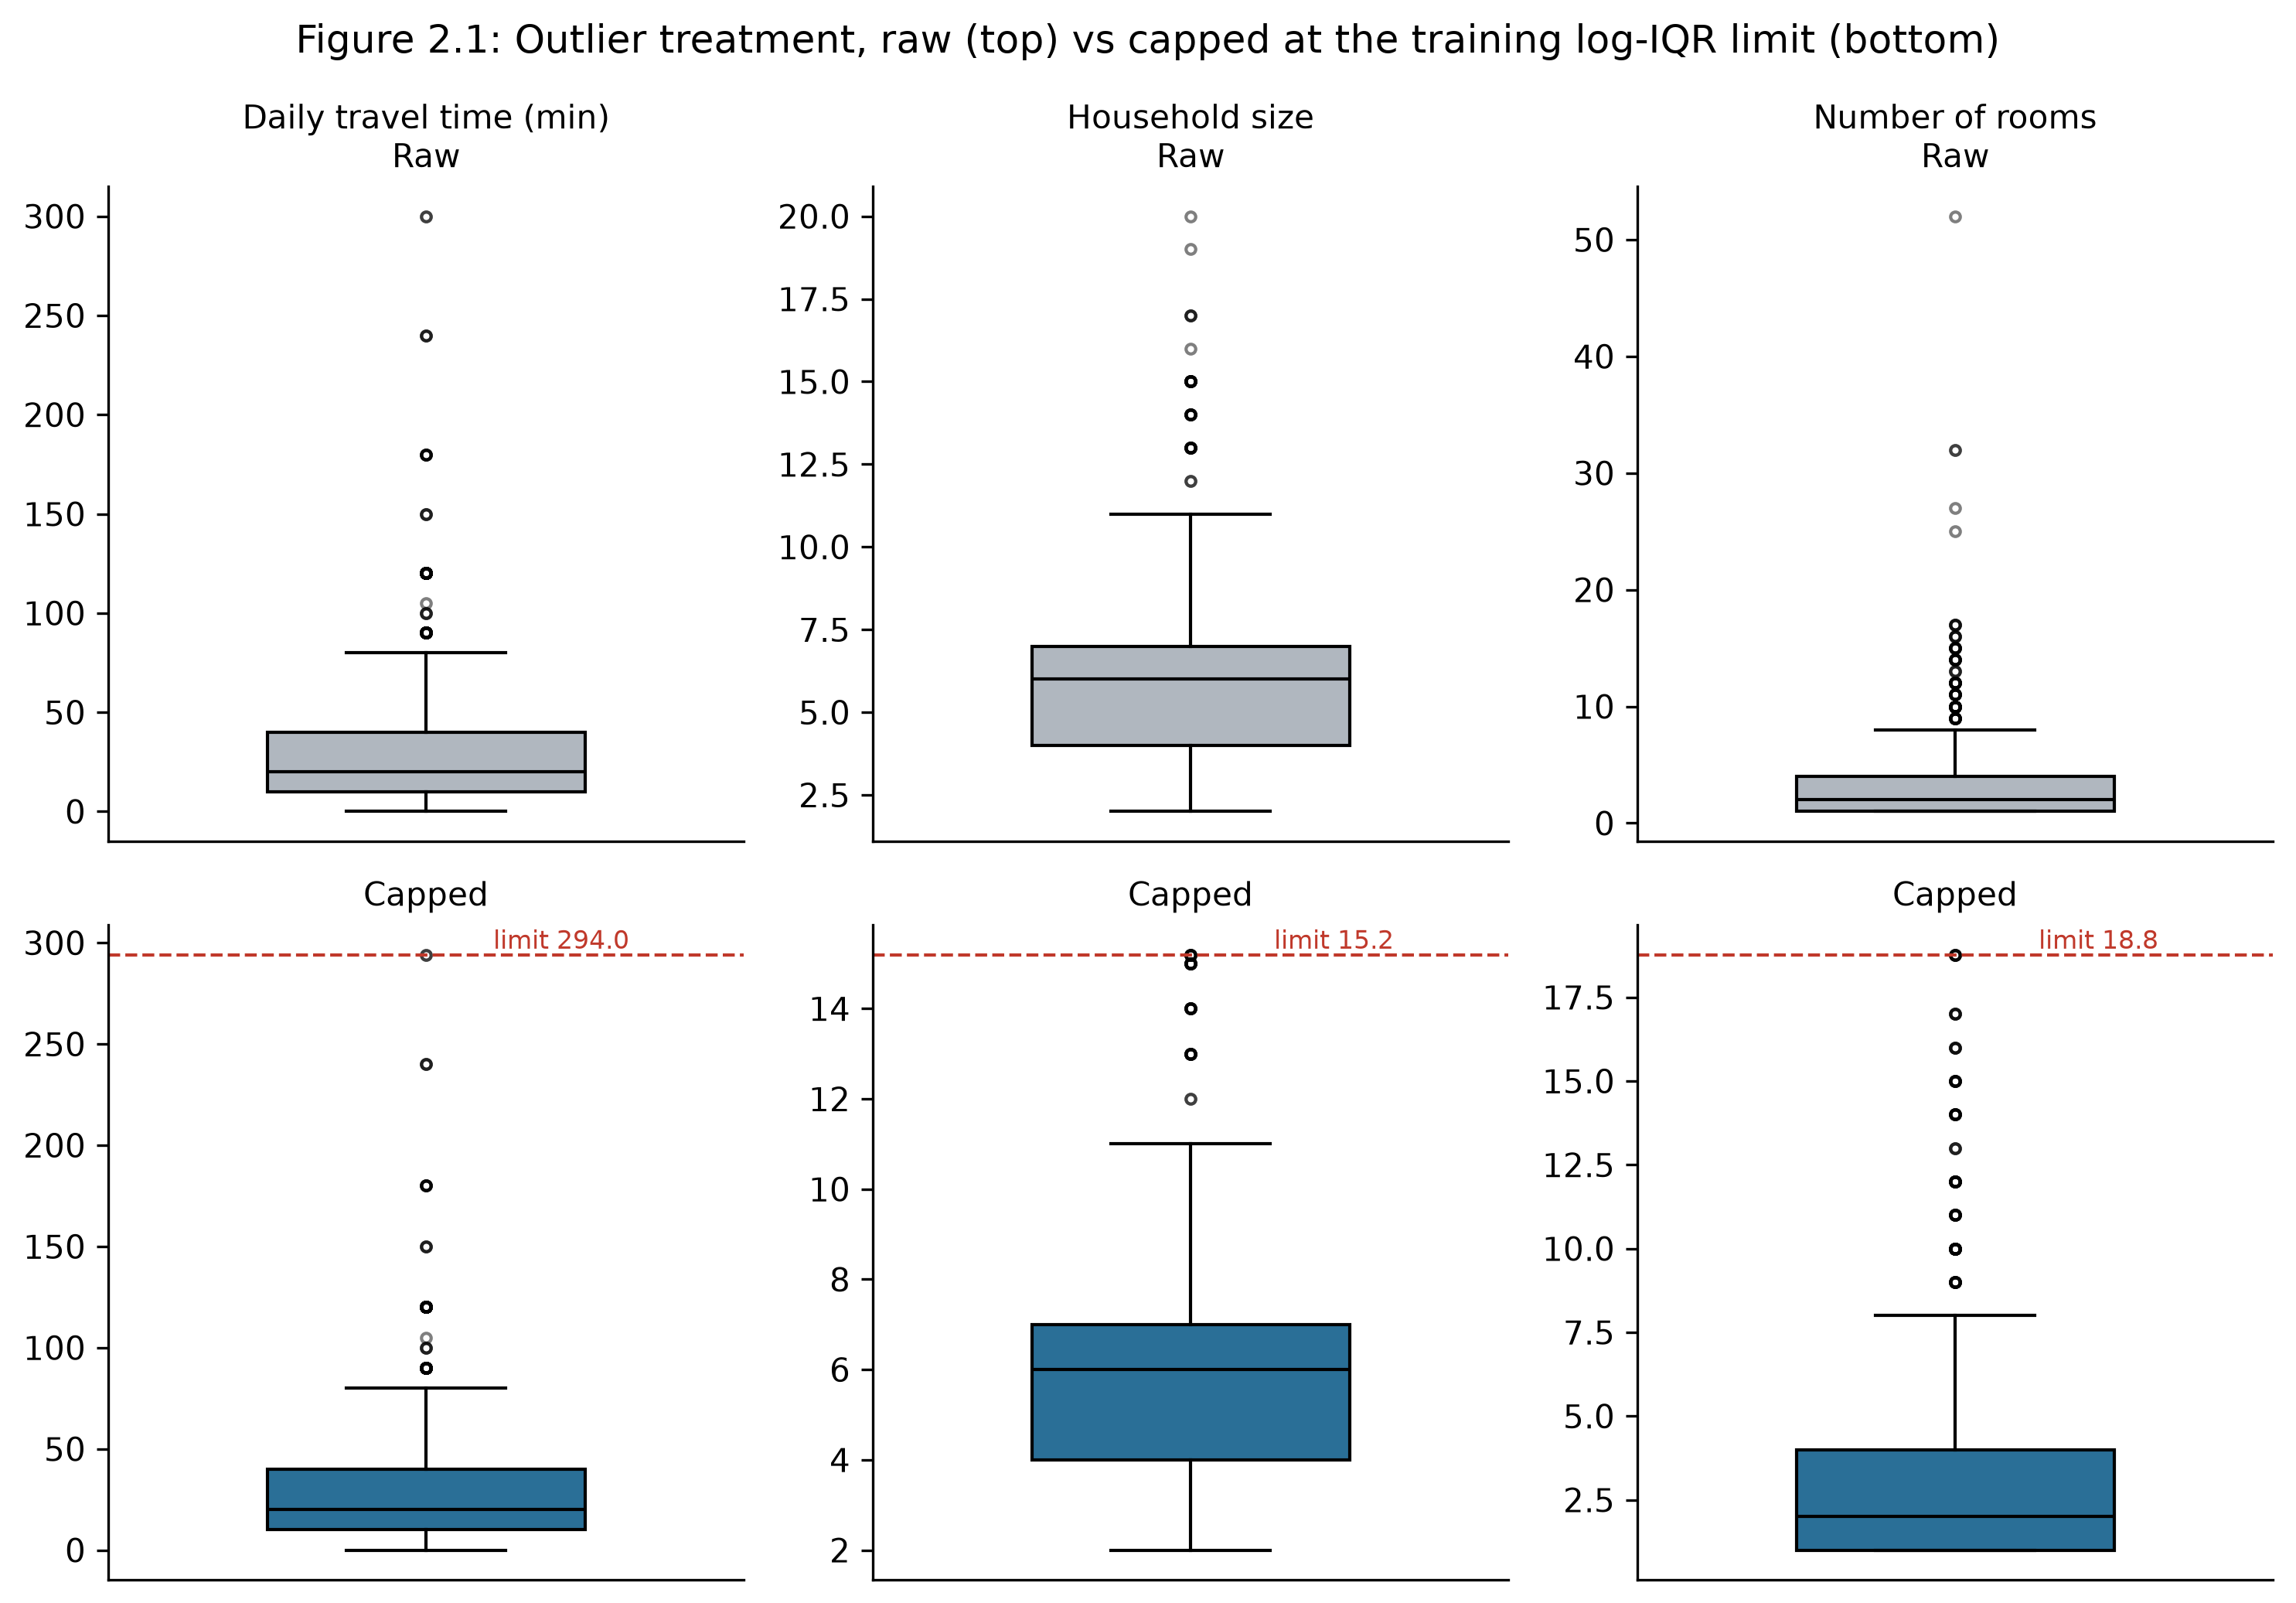
\includegraphics[width=0.72\textwidth]{fig2_1_outlier_boxplots.png}
\caption{Extreme values before (top) and after (bottom) capping, for the three capped features. \emph{How to read it:} the box holds the middle half of the children and the line inside it is the middle value; dots are unusually high values. The red dashed line is the limit learned from X\_train: 294.0 minutes, 15.2 people and 18.8 rooms. Values above the line are pulled down to it; no child is deleted.}
\label{fig:outliers}
\vspace{10pt}
\renewcommand{\thefigure}{3.1}
\centering
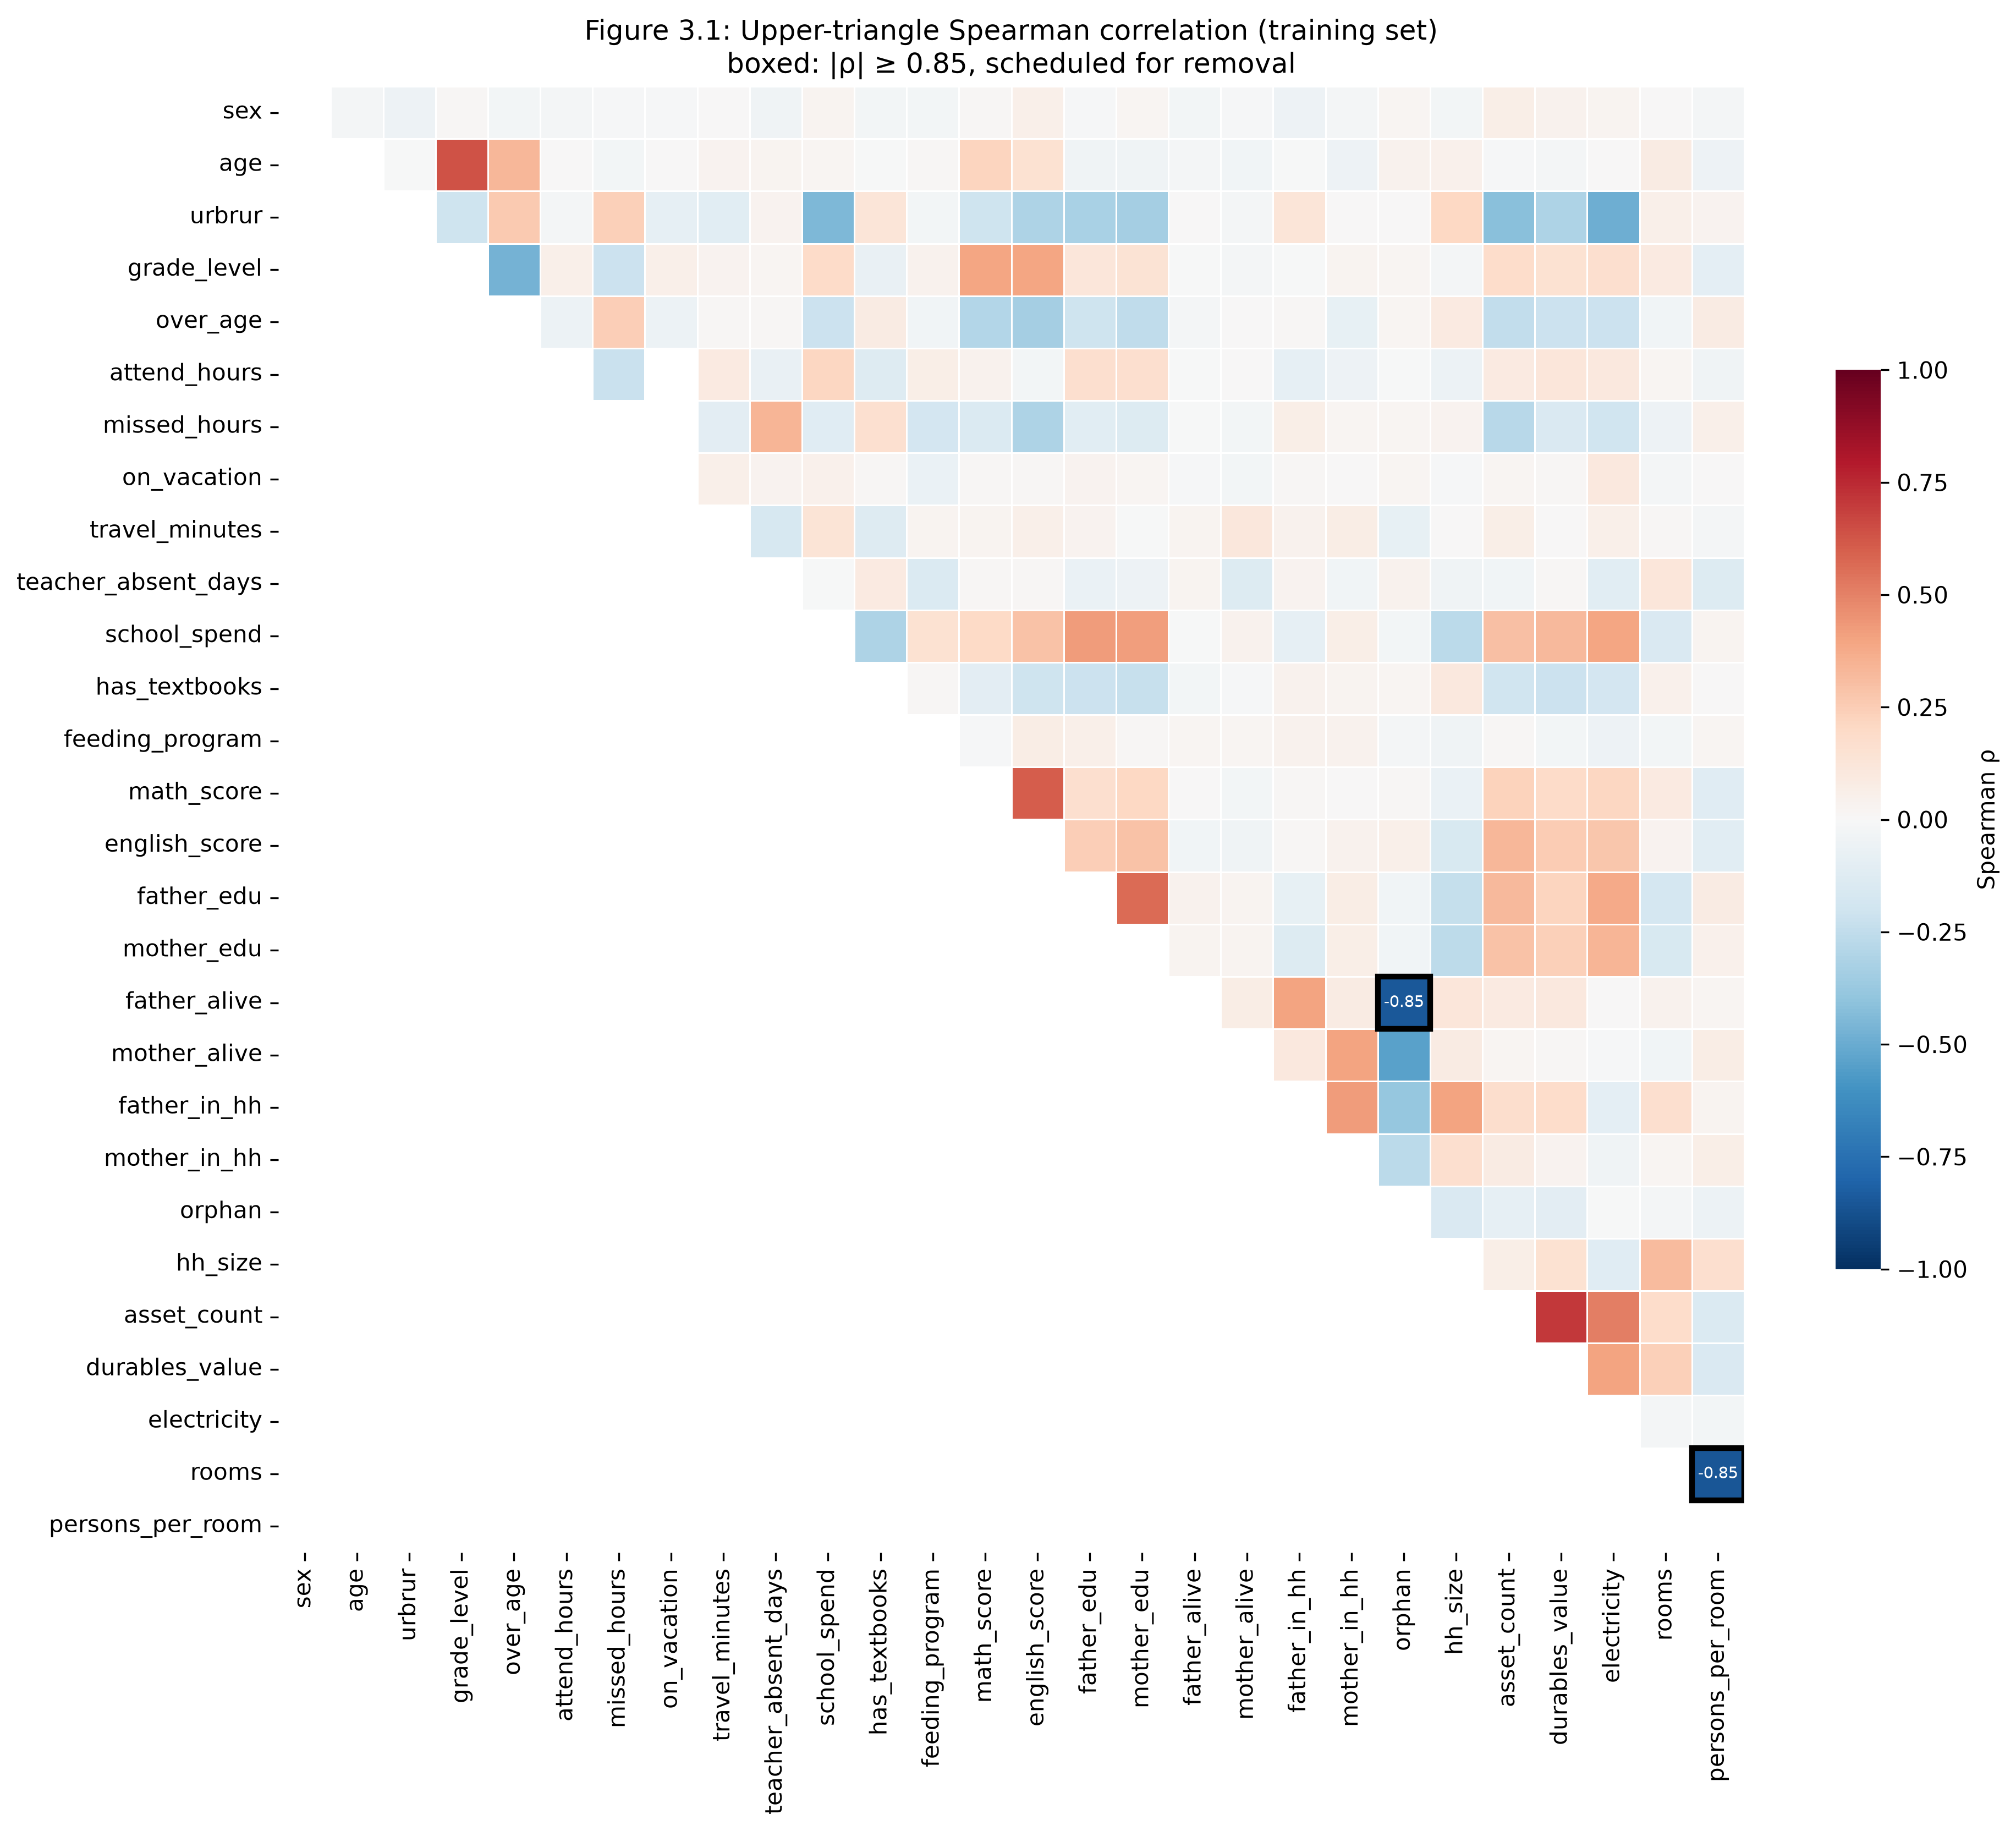
\includegraphics[width=0.6\textwidth]{fig3_1_correlation_matrix.png}
\caption{Which features repeat each other (rank correlation, X\_train). \emph{How to read it:} each square compares two features; dark red means they rise together, dark blue that one falls as the other rises. The two boxed squares are the pairs at or above 0.85 (ignoring the sign), which are scheduled for removal.}
\label{fig:corr}
\end{figure*}

\textbf{Extreme values (Fig.~\ref{fig:outliers}).} The limits learned by the pipeline (IQR rule on the log scale \cite{tukey}) are exactly those planned (294.0 minutes, 15.2 people, 18.8 rooms), and exactly 13 values are capped in X\_train (2 travel times, 6 household sizes, 5 room counts) and 5 in X\_test. The two money features are no longer shown: as planned in Phase 1, C1, they are ranked instead of capped, so their extreme values cannot dominate.

\begin{figure*}[p]
\renewcommand{\thefigure}{3.2}
\centering
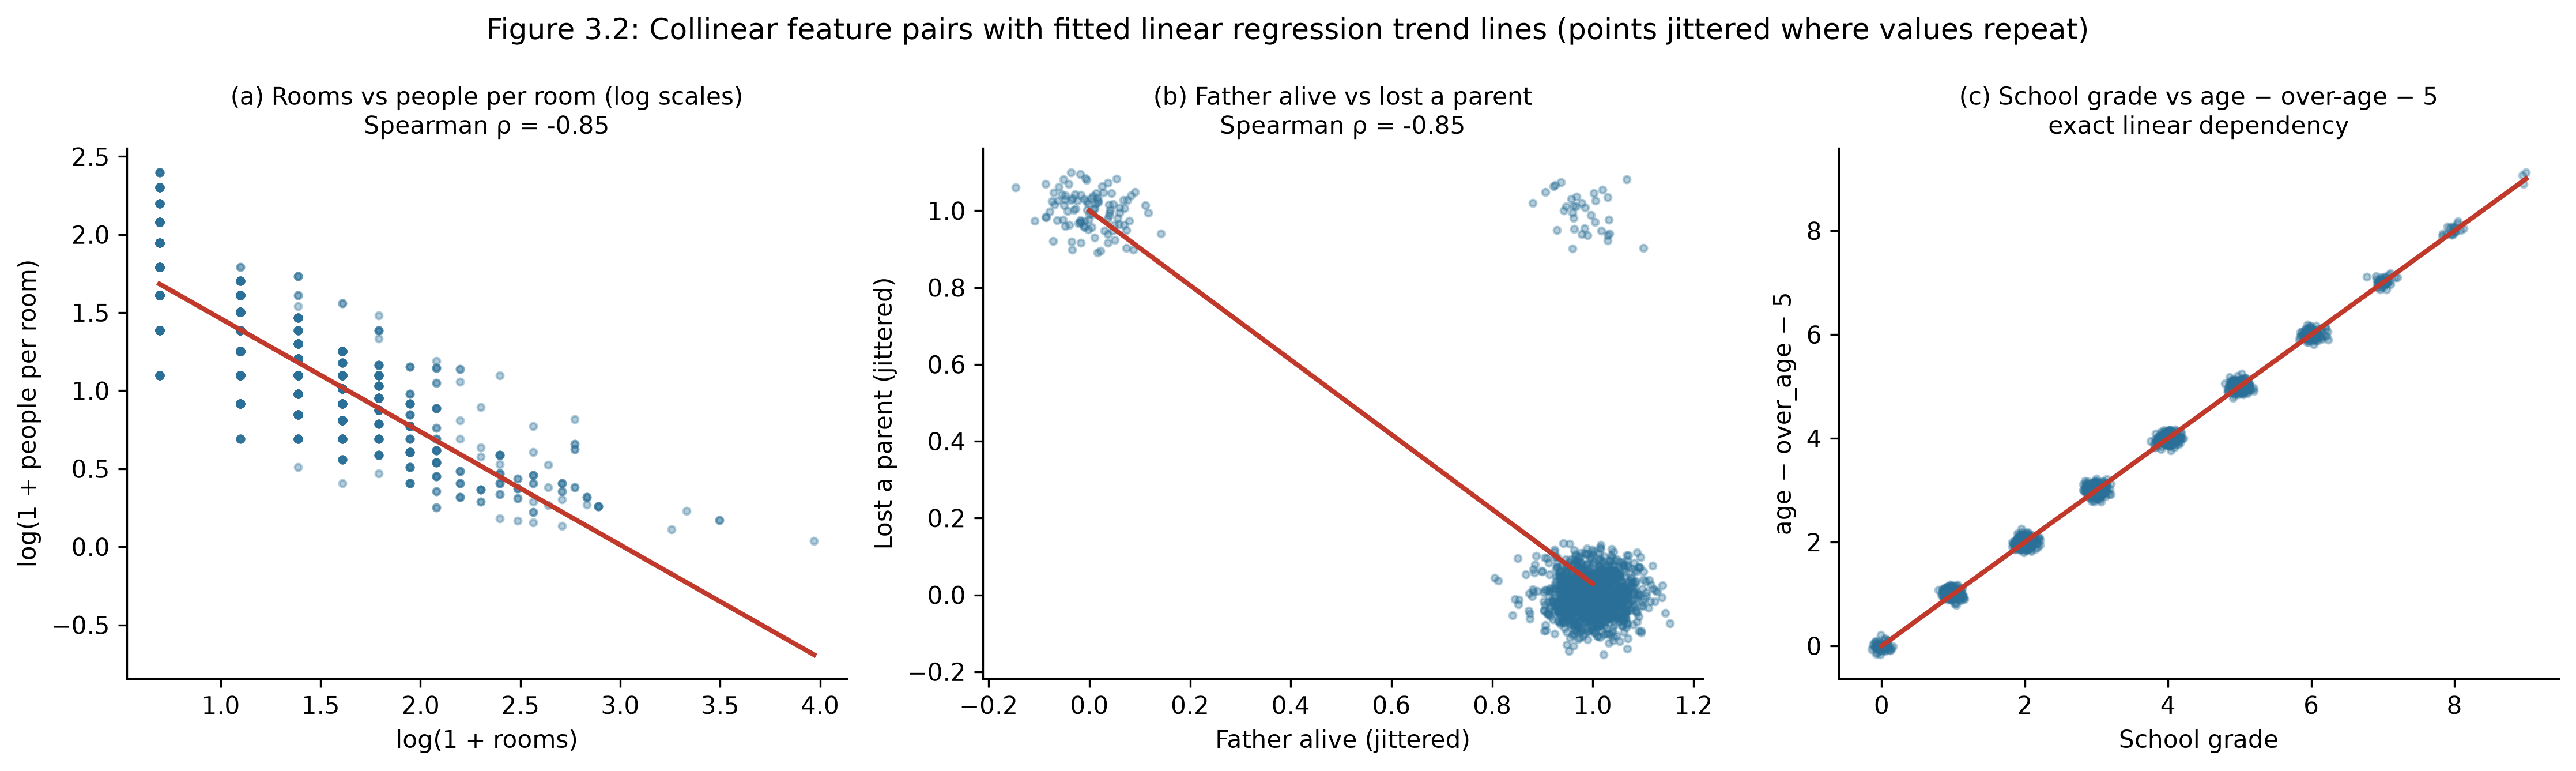
\includegraphics[width=0.92\textwidth]{fig3_2_collinear_scatterplots.png}
\caption{The three repeating features, one dot per child, with a fitted straight line. (a) More rooms, fewer people per room (log scales). (b) ``Lost a parent'' is almost the opposite of ``father alive'' (dots spread slightly so they do not sit on top of each other). (c) School grade equals age $-$ years over-age $-$ 5 for every child, so every dot lies on the line.}
\label{fig:collinear}
\vspace{8pt}
\renewcommand{\thefigure}{4.1}
\centering
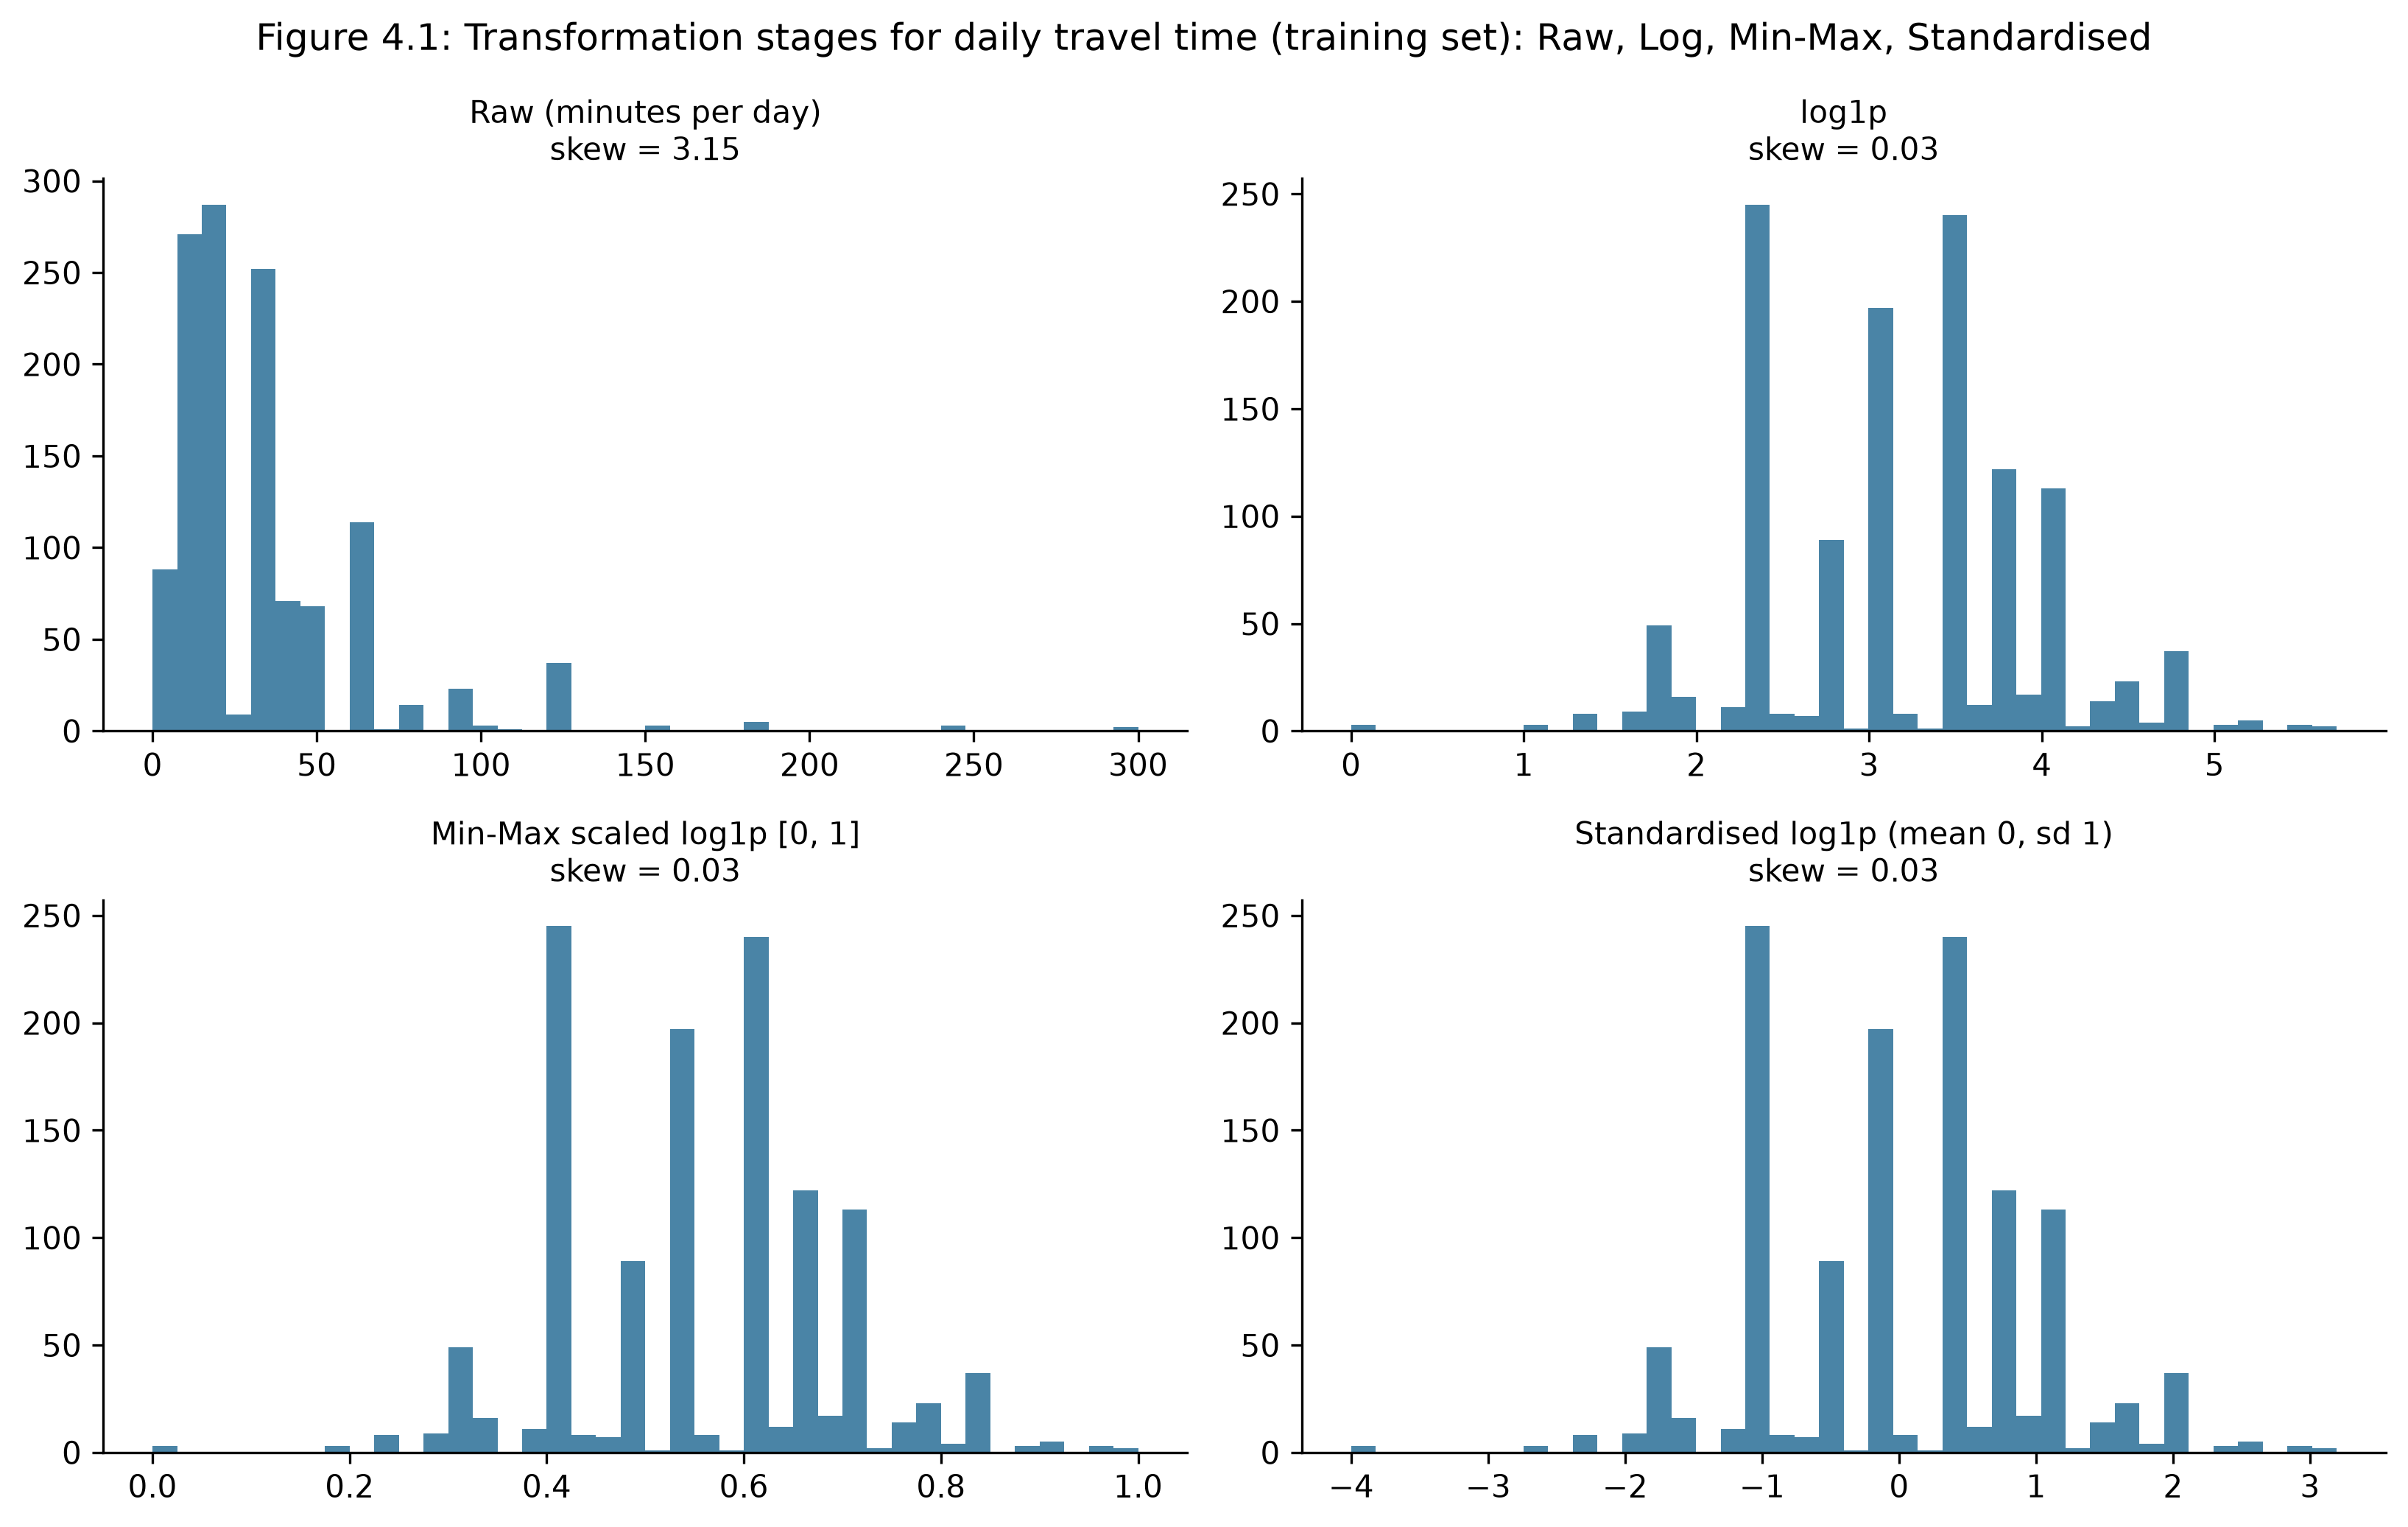
\includegraphics[width=0.64\textwidth]{fig4_1_transformation_grid.png}
\caption{What the transformation stages do to daily travel time (X\_train). Top left: raw minutes, with a long tail to the right (skew 3.15). Top right: after the log, the shape is balanced (skew 0.03). Bottom: the same logged values squeezed into 0--1 (Min--Max) and standardised (average 0, spread 1); the shape does not change, only the units on the bottom axis.}
\label{fig:transform}
\vspace{8pt}
\renewcommand{\thefigure}{5.1}
\centering
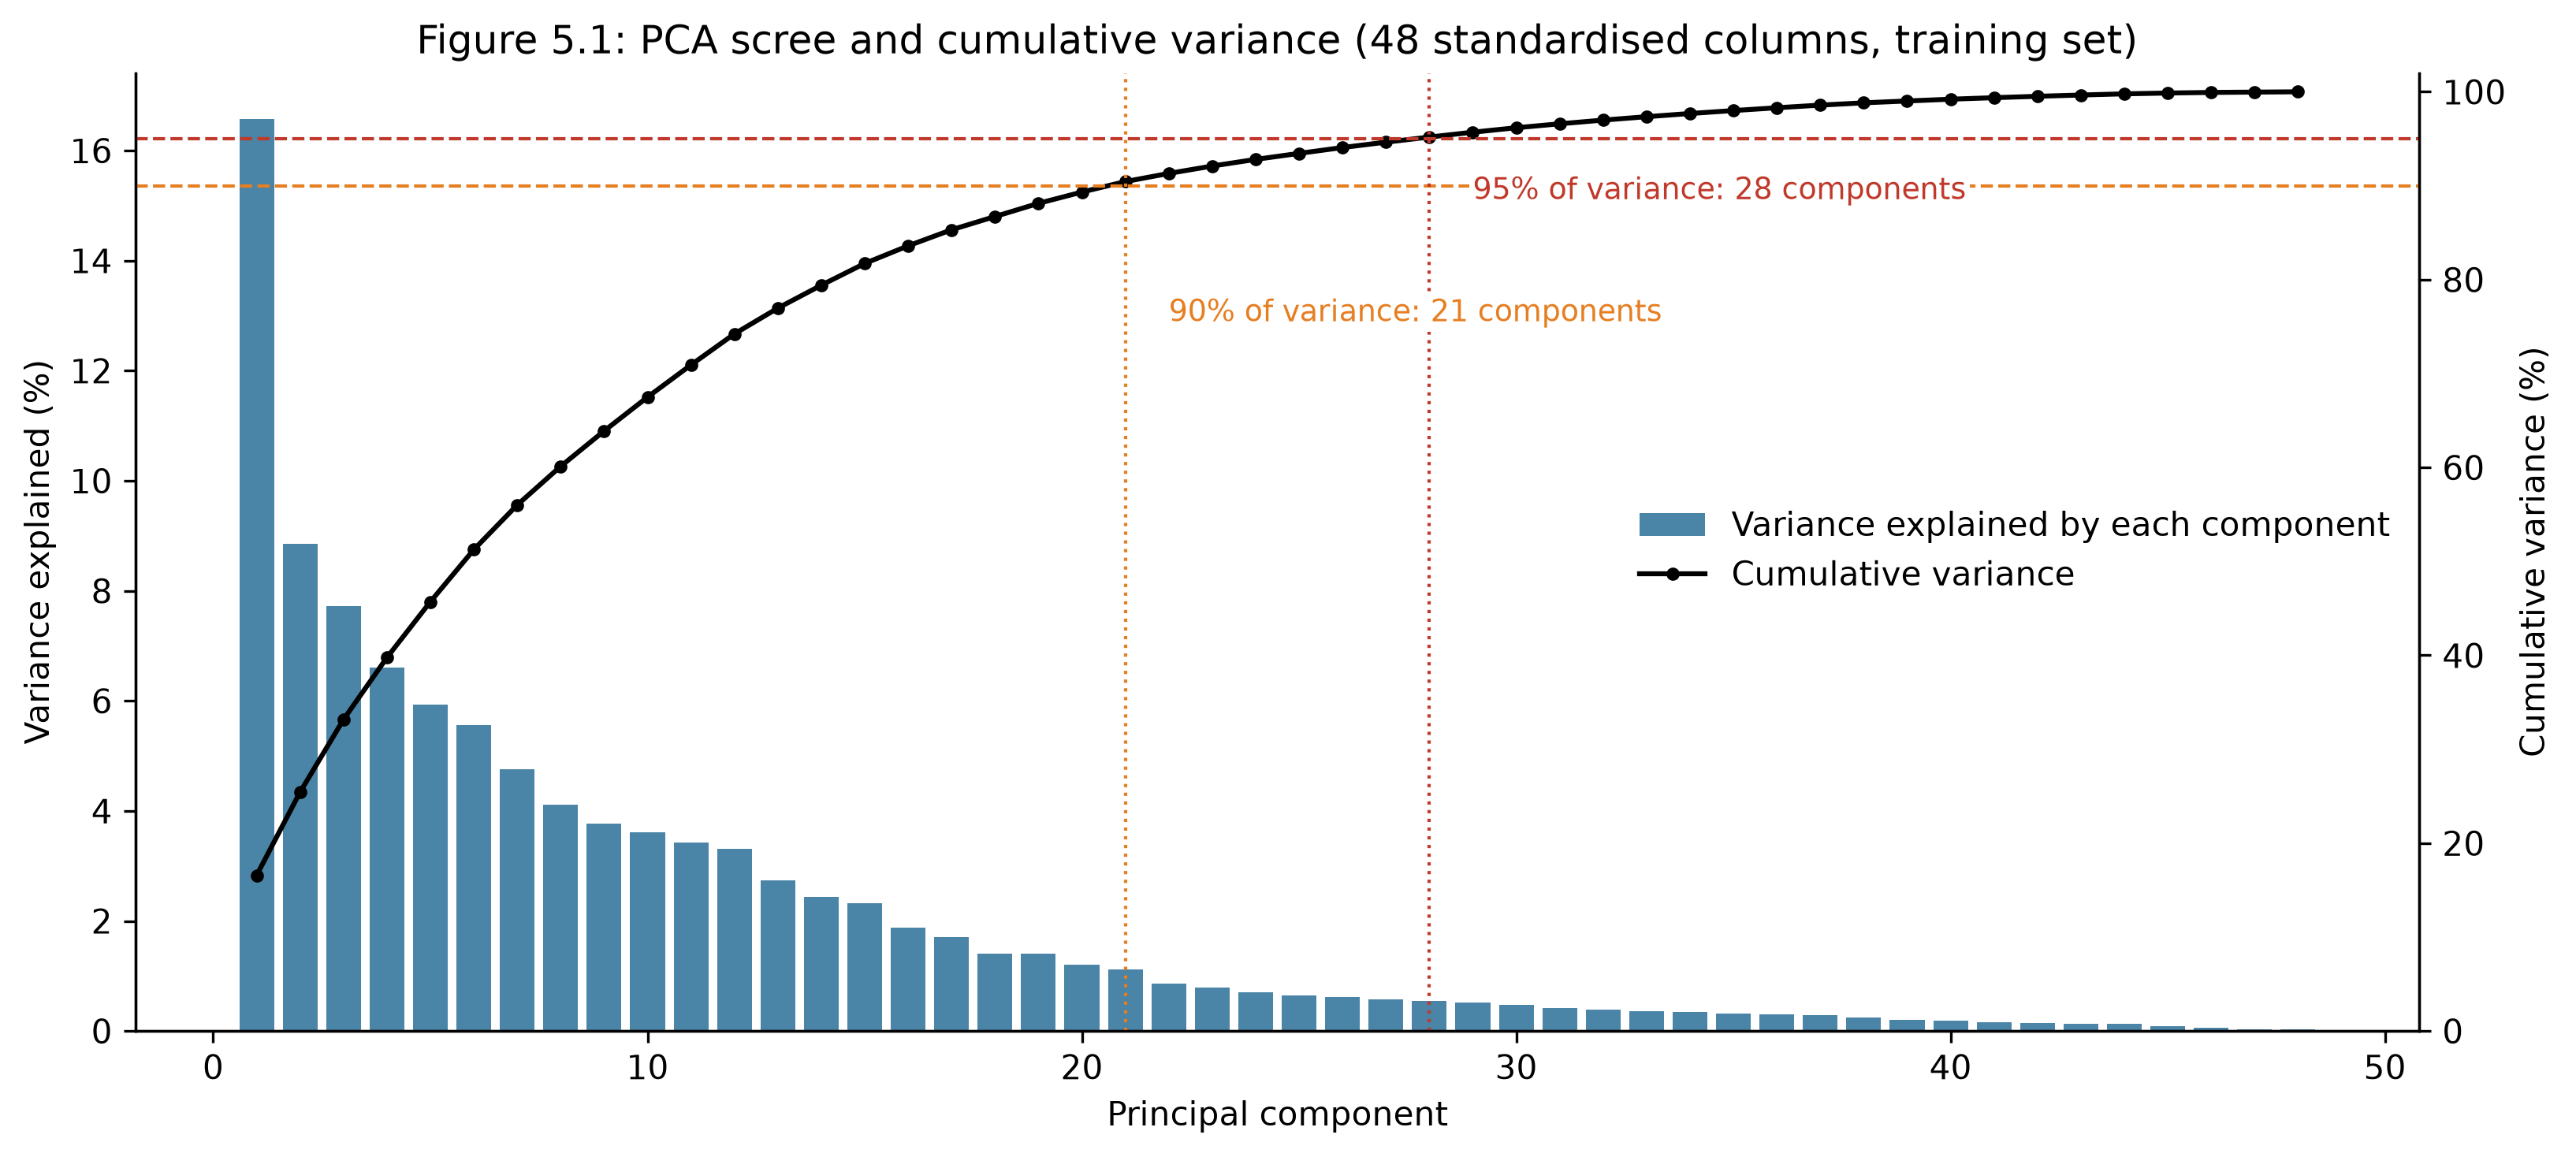
\includegraphics[width=0.8\textwidth]{fig5_1_pca_scree_plot.png}
\caption{Principal component analysis of the 48 standardised columns of X\_train. \emph{How to read it:} each bar is the share of the total variation captured by one combined component; the black line adds them up. The dashed lines mark 90\% and 95\% of the variation, reached with 21 and 28 components.}
\label{fig:pca}
\end{figure*}

\textbf{Repeating features (Figs.~\ref{fig:corr} and \ref{fig:collinear}).} The same two pairs are flagged as in Phase 1: father alive and lost a parent ($\rho=-0.850$), rooms and people per room ($\rho=-0.855$). The third case, school grade, is an exact calculation from age and years over-age (panel c). The fitted lines confirm that each removed feature follows directly from features that are kept.

\begin{figure}[!t]
\renewcommand{\thefigure}{3.3}
\centering
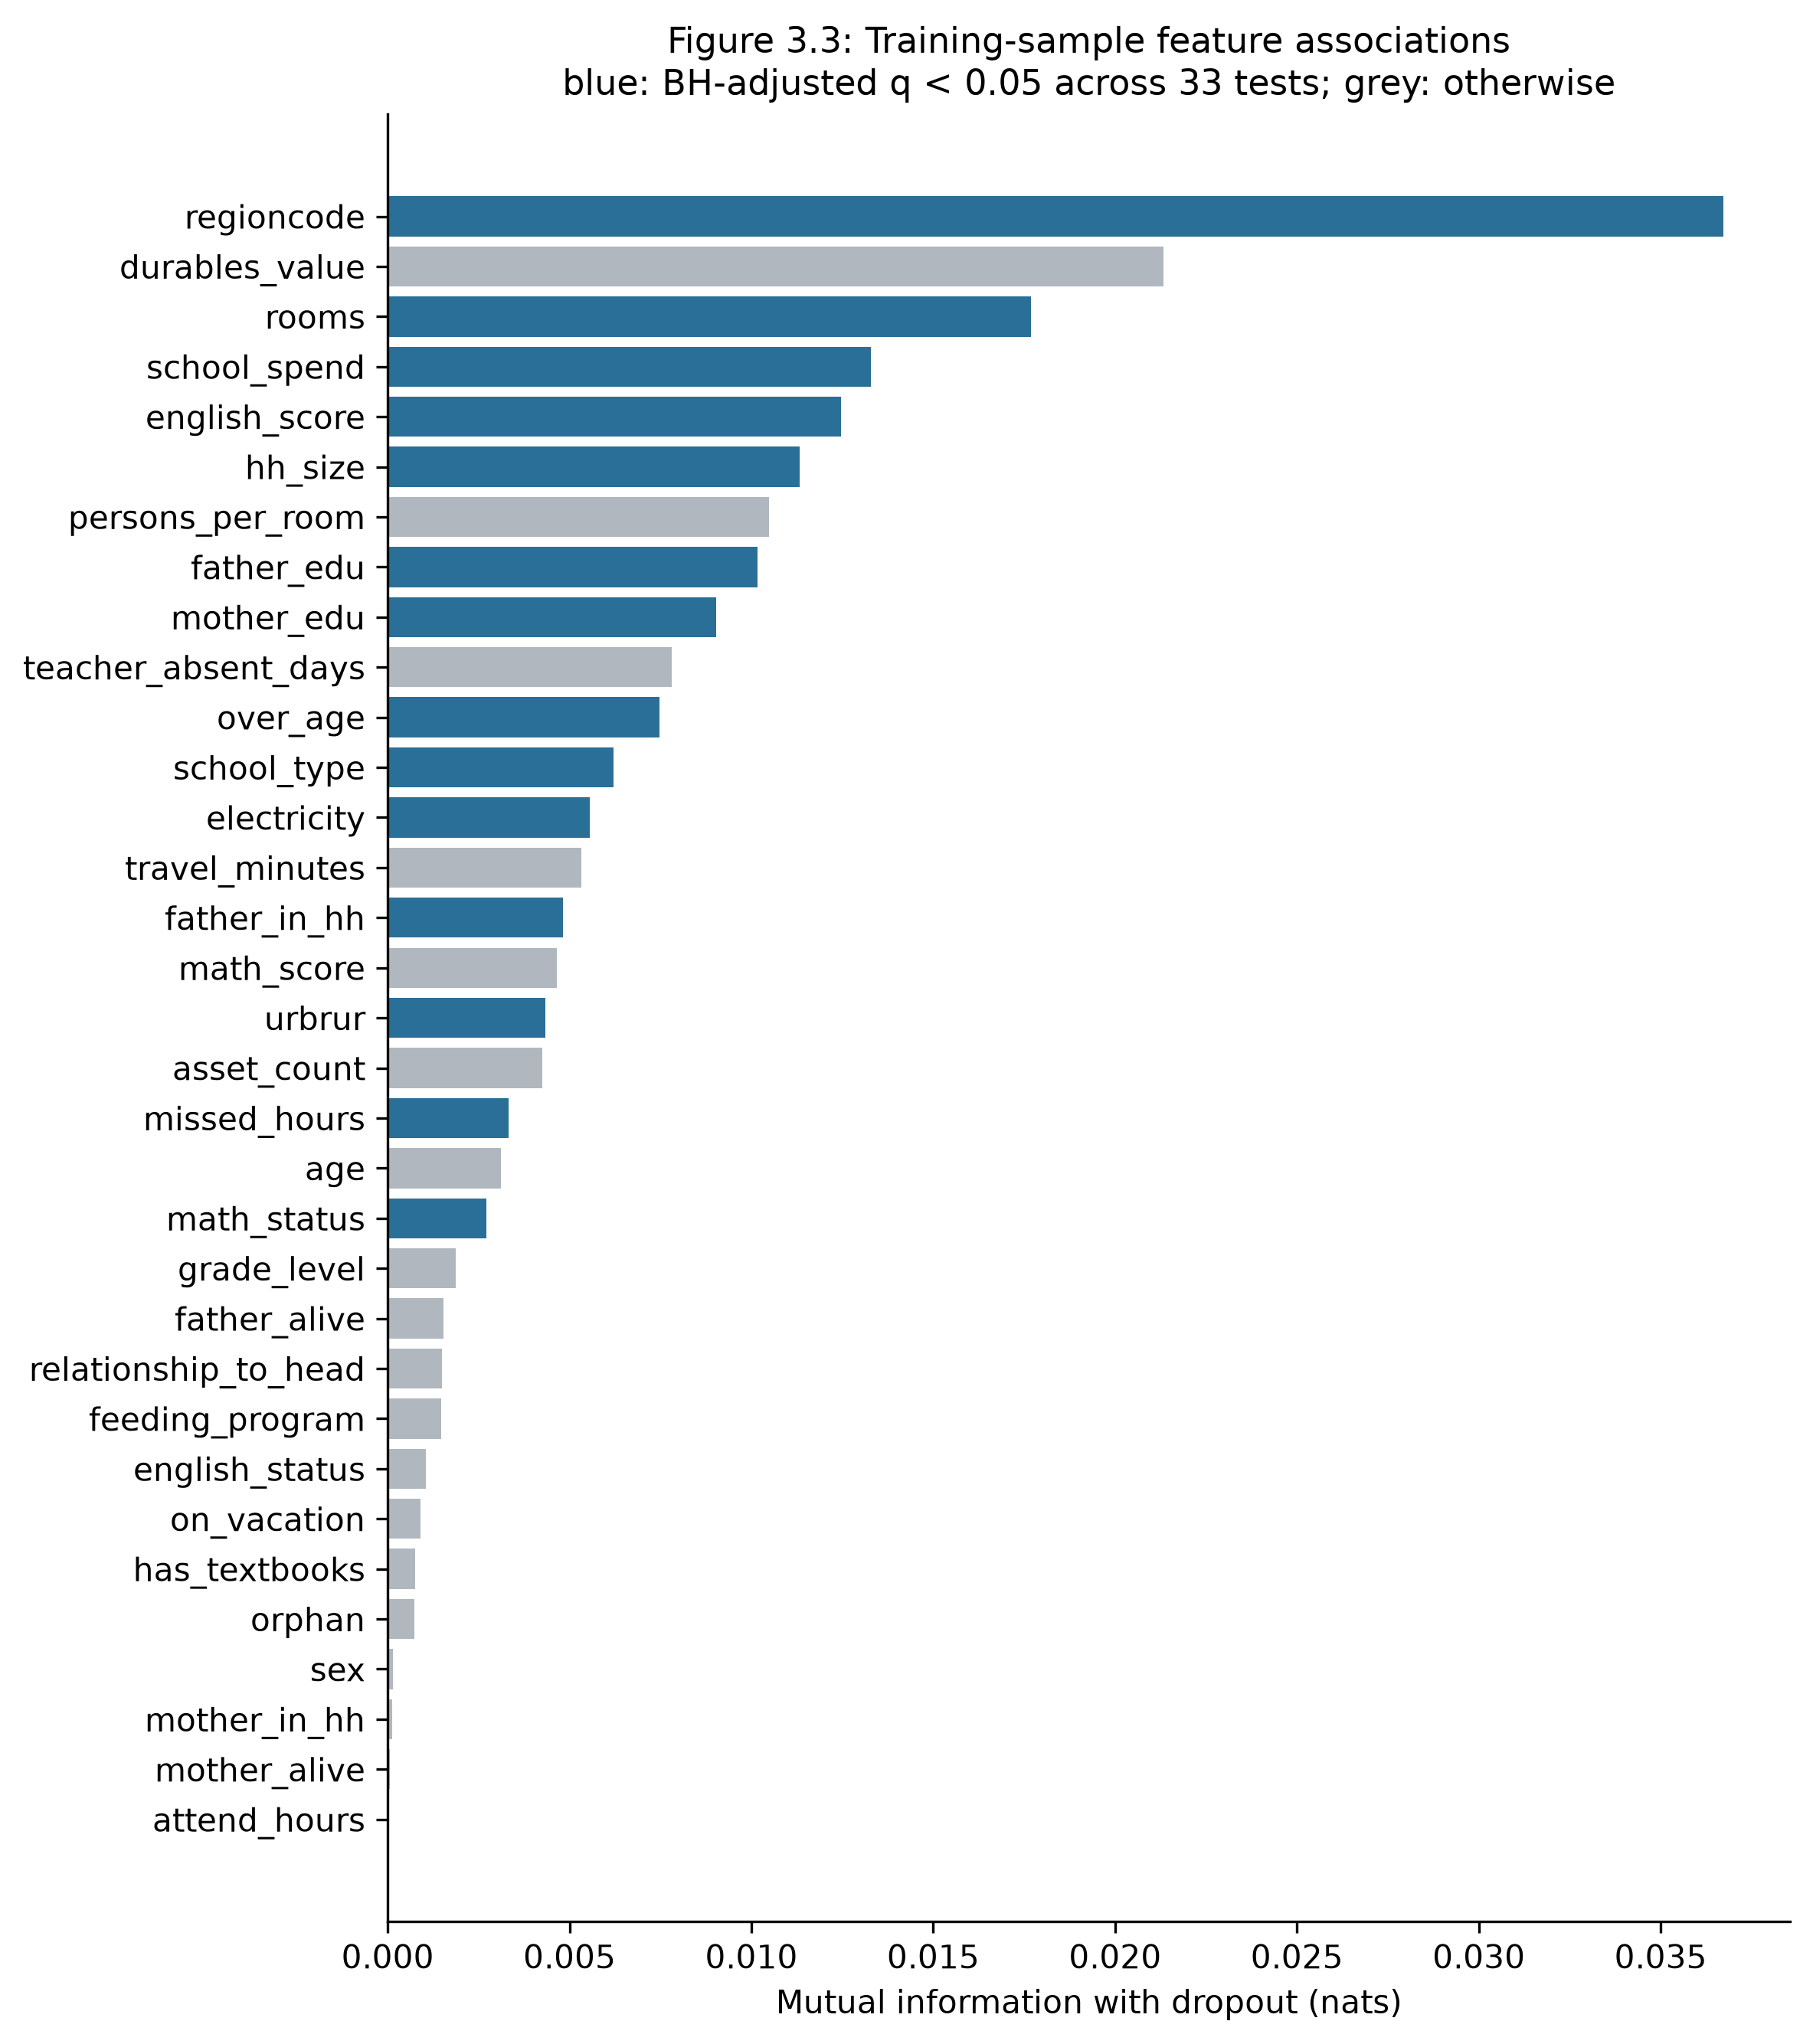
\includegraphics[width=0.85\columnwidth]{fig3_3_target_importance.png}
\caption{Which features tell us most about dropout (mutual information, X\_train). \emph{How to read it:} the longer the bar, the more the feature helps to tell dropouts from children who stay. Blue: the link is clear ($p<0.05$); grey: it could be chance.}
\label{fig:importance}
\end{figure}

\textbf{Links with dropout (Fig.~\ref{fig:importance}).} The ranking (mutual information \cite{kraskov}) is the one reported in Phase 1: region first (mutual information 0.037), then household goods, rooms, school spending, English score, household size and parents' education. No feature is removed for a weak link: choosing features belongs inside the folds of the modelling phase.

\textbf{Transformations (Fig.~\ref{fig:transform}).} The log is the step that changes the shape; Min--Max and standardising only change units. This confirms the Phase 1 choice: log on long tails, then \var{StandardScaler} for the simple model and PCA, and no rescaling for XGBoost.

\textbf{Dimension reduction (Fig.~\ref{fig:pca}).} The first component captures 16.6\% of the variation, and the curve then rises slowly: 21 of 48 components are needed for 90\% and 28 for 95\%. There is no small set of components that summarises the children well, so PCA would save little and would make the features harder to explain, which matters for an early-warning system whose warnings must be explained \cite{shap}. PCA is therefore kept as a diagnostic and not used to replace the features \cite{jolliffe}.

% ===============================================================
\section{Decision Log: Plan vs Implementation}
% ===============================================================
\begin{table*}[!t]
\centering
\caption{Decision log: every planned step from Phase 1 against what was built in Phase 2}
\label{tab:log}
\footnotesize
\setlength{\tabcolsep}{4pt}
\renewcommand{\arraystretch}{1.05}
\begin{tabularx}{\textwidth}{P{2.6cm} P{4.4cm} L P{2.9cm}}
\toprule
Step & Planned in Phase 1 & Implemented in Phase 2 (evidence) & Status \\
\midrule
Recording errors & Fixed rules for special codes and impossible values & Applied when the tables were built (\path{01_build_dataset.ipynb}); nothing learned & As planned \\
Inflation & Convert 2013/14 money to 2009/10 prices with the consumer price index & Factor 1.62 from World Bank data, weighted by the actual interview months & Adapted (Section V-A) \\
Split & By time; main test without the 220 children in both tables & X\_train 1,307; X\_test 1,395; main test 1,175 & As planned \\
Hours missed & Blank = 0 when attendance recorded; middle value otherwise; to be checked against a median fill & 756 blanks set to 0; 261 filled with the middle value; no measurable difference against a median fill & As planned, checked (V-C) \\
``Was missing'' flags & 4 flags, added before filling & Teacher absent, hours attended, father's and mother's education; compared between periods & As planned; limitation confirmed (V-D) \\
Filling gaps & Average / middle value / most common answer by skew; ``missing'' option for school type & \var{SimpleImputer} fitted on X\_train; 0 gaps left & As planned \\
School grade & 5 most similar children (KNN) on age, sex, urban, region, assets & 81 grades filled; years over-age recalculated, stays within $-3$ to 7 & As planned \\
Repeating features & Rank correlation $\ge0.85$ or VIF $>10$; drop 3; re-check inside each fold & Same pairs found; information-based choice matched the plan in 1 of 5 folds; tie-break rule decides; rebuilt exactly & Adapted (V-B) \\
Extreme values & Cap at the log-IQR limit; travel, household size, rooms & Limits 294.0, 15.2, 18.8; 13 capped (train), 5 (test); no child deleted & As planned \\
Money & Rank 0--1 against model-building values & \var{TrainingRank} fitted on X\_train & As planned; new finding (V-A) \\
Encoding & One-hot (labels), ordered numbers, 0/1 & 53 columns (XGBoost), 48 (logistic regression) & As planned \\
Scaling & None for XGBoost; log + \var{StandardScaler} for logistic regression and PCA & As planned; PCA: 21 components for 90\%, 28 for 95\% & As planned \\
Correlation measure & Rank (Spearman) correlation, because no feature is bell-shaped & Ordinary (Pearson) correlation would have missed one pair & Confirmed (V-E) \\
Cross-validation & 5 folds, same dropout share, whole districts & \path{StratifiedGroupKFold}; 0 shared districts or households & As planned \\
Fewer dropouts & Extra weight on dropouts, recalculated in each fold & \var{scale\_pos\_weight}; \path{class_weight="balanced"} & As planned \\
Calibration, final test & Calibrate on checking folds; test once & Not run in Phase 2: they belong to the modelling phase & Deferred \\
\bottomrule
\end{tabularx}
\tabnote{The same table is saved by the notebook as \path{phase2_implementation/decision_log.csv}.}
\end{table*}

Table~\ref{tab:log} tracks every planned item. Of the 16 steps, 10 were built exactly as planned, 2 were checked and confirmed (hours missed, correlation measure), 1 confirmed a limitation (flags), 2 were adapted (inflation, choice of repeating feature) and 1 is deferred to the modelling phase (calibration and the final test). The changes are explained in Section~V.

% ===============================================================
\section{Deviations and Rationale}
% ===============================================================
\subsection{Inflation explains only about half of the money rise}
\textbf{Plan.} Phase 1 said the typical value of household goods was 2.56 times higher in 2013/14 ``mostly because of inflation''. \textbf{Reality.} Prices rose by a factor of 1.62 between the two visits, so inflation explains only about half of the rise (on a log scale, $\ln 1.62/\ln 2.56 \approx 0.51$). After the adjustment, the typical testing child sits at rank 0.63 of the 2009/10 household-goods values, not 0.50: households really did own more. School spending moved the other way: the typical testing child sits at rank 0.39, so real spending on schooling fell, which is consistent with Ghana's fee-free schooling policies. \textbf{Decision.} Keep the plan (convert to 2009/10 prices, then rank against model-building values \cite{filmer2001}). The ranks now carry these real changes instead of hiding them, which is what a model used in a later period needs to see. The check promised in Phase 1 (ranking within the 2013/14 survey itself) is left for the modelling phase, where it can be compared on test results.

\subsection{Which repeating feature to drop is not stable across folds}
\begin{table}[!t]
\centering
\caption{Re-check of the repeating features inside each fold}
\label{tab:folds}
\footnotesize
\setlength{\tabcolsep}{3pt}
\begin{tabular}{crrlll}
\toprule
Fold & \makecell{$\rho$ rooms /\\people} & \makecell{$\rho$ father /\\lost parent} & \makecell[l]{Less info,\\pair 1} & \makecell[l]{Less info,\\pair 2} & \makecell[l]{Least info,\\group 3} \\
\midrule
1 & $-0.851$ & $-0.842$ & people/room & lost parent & grade \\
2 & $-0.861$ & $-0.831$ & rooms & lost parent & grade \\
3 & $-0.854$ & $-0.861$ & rooms & lost parent & grade \\
4 & $-0.858$ & $-0.854$ & people/room & father alive & age \\
5 & $-0.850$ & $-0.866$ & rooms & lost parent & age \\
\bottomrule
\end{tabular}
\tabnote{Computed on the building part of each fold only. Group 3 = age, grade and years over-age. Full table: section 7 of the notebook.}
\end{table}

\textbf{Plan.} Phase 1 dropped, in each repeating pair, the feature with less information about dropout, and promised to re-check this inside each fold. \textbf{Reality.} Table~\ref{tab:folds} shows that the relationships themselves are stable (all correlations between $-0.83$ and $-0.87$, and the age, grade and over-age calculation is exact), but the feature with less information changes from fold to fold. The plan's choice was reproduced in only 1 of 5 folds. The reason is that the differences in mutual information are tiny (for example 0.0008 vs 0.0015 for lost a parent vs father alive) and smaller than the variation between folds. \textbf{Decision.} Phase 1 already gave the rule for this case: ``if similar, keep the one measured directly over one calculated from others''. People per room (calculated from household size and rooms) and lost a parent (calculated from the two parent-alive items) are therefore removed. In the age, grade and over-age group, years over-age is kept because it is the risk signal behind the project's central idea, and age because it is measured directly; grade is removed. The list is fixed before cross-validation, so it cannot be tuned on the checking parts. Since each removed feature can be rebuilt exactly (Section~VI), no information is lost whichever member is kept.

\subsection{Hours missed: the rule and a median fill perform the same}
\textbf{Plan.} Fill a blank ``hours missed'' with 0 when attendance was recorded, and check this against a median fill. \textbf{Reality.} The rule sets 756 blanks to 0; 261 blanks remain (interviews in school holidays) and get the middle value. In the five-fold check the two versions give the same result within noise (logistic regression PR-AUC 0.265 vs 0.274; XGBoost 0.255 vs 0.257, with a fold-to-fold spread of about $\pm0.08$). The share of children reporting some hours missed, when attendance was recorded, is 15.7\% in 2009/10 and 14.4\% in 2013/14, which supports the rule. \textbf{Decision.} Keep the rule: it does not hurt the model and it matches what a blank on the paper form most likely meant, so the feature has the same meaning in both periods.

\subsection{``Was missing'' flags mean different things in the two periods}
The share of children with each flag switched on is about half as large in 2013/14 as in 2009/10: teacher absent 56.8\% vs 31.8\%, hours attended 21.8\% vs 11.7\%, father's education 7.7\% vs 5.4\%, mother's education 3.8\% vs 1.9\%. Tablets that required an answer explain most of this. This confirms the limitation stated in Phase 1: a flag learned from 2009/10 may not mean the same thing in a later period. The flags are kept, because the gap is informative inside each period (for teacher absence it is linked to dropout, 17.2\% vs 10.6\%), and their effect will be compared between periods when models are evaluated.

\subsection{Rank correlation was needed, not the ordinary one}
The assignment's screening rule is written as $|r|\ge0.85$. Because no feature is bell-shaped, Phase 1 used the rank (Spearman) correlation $\rho$ with the same threshold. Phase 2 shows why this mattered: for rooms and people per room, $\rho=-0.855$ but the ordinary (Pearson) correlation is only $r=-0.563$, because the relationship is curved (people per room = household size / rooms). With Pearson $r$, this repeating pair would have been missed, and the VIF check also misses it (VIF 1.77). For father alive and lost a parent, both measures give $-0.850$.

% ===============================================================
\section{Pipeline Output Verification}
% ===============================================================
\begin{table}[!t]
\centering
\caption{Size of the data at each stage}
\label{tab:dims}
\footnotesize
\setlength{\tabcolsep}{4pt}
\begin{tabularx}{\columnwidth}{L r r}
\toprule
Stage & X\_train & X\_test \\
\midrule
Children (rows) & 1,307 & 1,395 \\
Features before the pipeline & 33 & 33 \\
Features after removing 3 repeating ones & 30 & 30 \\
Columns, XGBoost version & 53 & 53 \\
Columns, logistic regression / PCA version & 48 & 48 \\
Missing values after the pipeline & 0 & 0 \\
Children deleted & 0 & 0 \\
\bottomrule
\end{tabularx}
\tabnote{53 = 16 numbers or ordered numbers + 9 yes/no items + 24 yes/no columns from the label options + 4 ``was missing'' flags. The logistic regression version leaves out one option for each of the 5 labels (53 $-$ 5 = 48).}
\end{table}

\begin{table}[!t]
\centering
\caption{No information lost: rebuilding the removed features}
\label{tab:rebuild}
\footnotesize
\setlength{\tabcolsep}{3pt}
\begin{tabularx}{\columnwidth}{P{1.9cm} L r r}
\toprule
Removed & Rebuilt from kept features & \makecell{Children\\checked} & \makecell{Children\\that differ} \\
\midrule
School grade & age $-$ years over-age $-$ 5 & 1,226 & 0 \\
Lost a parent & 1 if father or mother has died & 1,279 & 0 \\
People per room & household size / rooms & 1,302 & 0 \\
\bottomrule
\end{tabularx}
\tabnote{All children of X\_train with the needed values recorded; 3,807 checks in total.}
\end{table}

\textbf{Final size.} Table~\ref{tab:dims} confirms that the pipeline produces exactly the size planned in Phase 1: 33 features become 30, then 53 columns for XGBoost and 48 for logistic regression, for every child of X\_train and X\_test, with no missing value and no child deleted.

\textbf{Feature count reduced without information loss.} The assignment asks for proof that the reduction from 33 to 30 loses no information. Table~\ref{tab:rebuild} rebuilds each removed feature from features that are kept and compares the result with the original value for every child. The rebuilt value is identical in all 3,807 checks. The three removed features therefore add nothing that the model cannot already see.

\textbf{No leakage.} (1) Every learned setting is fitted on X\_train only; the notebook confirms that applying the pipeline to X\_test leaves its fitted settings unchanged. (2) In cross-validation the whole pipeline is re-fitted on the building part of each fold; no district or household is shared between building and checking parts. (3) The outcomes of X\_test are not used in this phase.

\begin{table}[!t]
\centering
\caption{Quick end-to-end check (5 district-grouped folds, X\_train)}
\label{tab:cv}
\footnotesize
\setlength{\tabcolsep}{4pt}
\begin{tabular}{lrr}
\toprule
Model (untuned) & PR-AUC & ROC-AUC \\
\midrule
Logistic regression (48 columns) & 0.265 ($\pm$0.072) & 0.626 \\
XGBoost (53 columns) & 0.255 ($\pm$0.088) & 0.600 \\
No skill (dropout rate) & 0.144 & 0.500 \\
\bottomrule
\end{tabular}
\tabnote{Mean ($\pm$ spread) over the 5 checking parts. Both models are untuned; this only shows that the full pipeline runs and finds real signal.}
\end{table}

\textbf{The pipeline works end to end.} Table~\ref{tab:cv} shows that both untuned models, trained through the full pipeline fold by fold, rank real dropouts well above chance (PR-AUC \cite{saito2015}, about 0.25--0.27 against 0.144 for no skill). The numbers are modest, as expected before tuning and with folds made of whole districts, which stops a model from relying on local patterns it has already seen. The processed tables are saved as \path{data/processed/train_processed_xgb.csv} and \path{test_processed_xgb.csv} (53 columns plus identifiers and the outcome) and the matching \var{\_lr} files (48 columns); the test files mark the 220 children who appear in both tables.

% ===============================================================
\section{Limitations and Next Steps}
% ===============================================================
\begin{itemize}\setlength{\itemsep}{0pt}
\item \textbf{Change over time.} Dropout fell from 14.4\% to 10.4\%, regional patterns changed, household goods rose in real terms and school spending fell. A model built on 2009/10 may overstate risk in the later period; this will be measured on the single final test.
\item \textbf{Flags across periods.} The ``was missing'' flags are switched on about half as often in 2013/14 (Section~V-D); their weight in the model will be compared between periods.
\item \textbf{Children who could not be found again.} As reported in Phase 1, they share known dropout risk factors, so the true dropout rate is probably understated; the sensitivity check on the identity rule (age change of 1--8 years) is part of the modelling phase.
\item \textbf{Next steps (modelling phase).} Tune both models inside the same folds, adjust the risk percentages (calibration) on the checking parts, choose the cut-off for flagging the riskiest 20\%, and then test once on X\_test, with and without the 220 children who appear in both tables.
\end{itemize}

% ===============================================================
\clearpage
\section*{Appendix: Plain-Language Guide to the Technical Terms}
The terms below are used in this report; terms already explained in the Phase 1 report keep the same meaning.

{\footnotesize
\noindent\textbf{Pipeline:} A chain of preparation steps followed by a model, run in a fixed order. Fitting it learns every setting from the training data at once.\par\vspace{2pt}
\noindent\textbf{ColumnTransformer:} The part of the pipeline that applies the right preparation to each group of columns side by side (for example, a middle-value fill for lopsided numbers and one-hot encoding for labels).\par\vspace{2pt}
\noindent\textbf{Fit / transform:} \emph{Fit} = learn the settings (e.g.\ a middle value or a cap limit) from data; \emph{transform} = apply the stored settings to any data without learning anything new.\par\vspace{2pt}
\noindent\textbf{X\_train / X\_test:} The children used to build the model (2009/10) and the children kept aside to test it (2013/14).\par\vspace{2pt}
\noindent\textbf{Leakage:} When information from the data used for checking sneaks into building the model, making results look better than they really are.\par\vspace{2pt}
\noindent\textbf{Fold, building part, checking part:} Cross-validation splits X\_train into 5 parts; the model is built on 4 (the building part) and checked on the 5th (the checking part), rotating 5 times.\par\vspace{2pt}
\noindent\textbf{Custom transformer:} A preparation step written for this project (in \path{src/transformers.py}) that follows the same fit / transform rules as the standard scikit-learn steps.\par\vspace{2pt}
\noindent\textbf{KNN (nearest neighbours) filling:} Filling a missing value using the 5 most similar children in the training data.\par\vspace{2pt}
\noindent\textbf{Capping:} Pulling an extreme value down to a set limit instead of deleting the child.\par\vspace{2pt}
\noindent\textbf{Rank (0--1):} The position of a value among the training values: 0 = lowest, 0.5 = middle, 1 = highest.\par\vspace{2pt}
\noindent\textbf{Consumer price index, inflation factor:} The official measure of how prices rise; dividing 2013/14 amounts by 1.62 expresses them in 2009/10 prices.\par\vspace{2pt}
\noindent\textbf{One-hot encoding:} Turning a label with several options (e.g.\ 10 regions) into separate yes/no columns.\par\vspace{2pt}
\noindent\textbf{Standardising:} Putting numbers on a common scale with average 0 and spread 1.\par\vspace{2pt}
\noindent\textbf{Correlation ($r$, $\rho$):} How closely two features move together, from $-1$ to $+1$. The ordinary (Pearson) $r$ only sees straight-line relationships; the rank (Spearman) $\rho$ also sees curved ones.\par\vspace{2pt}
\noindent\textbf{VIF:} How much a feature is already explained by all the others together (above 10 = redundant).\par\vspace{2pt}
\noindent\textbf{Mutual information:} How much knowing a feature reduces uncertainty about dropout; it captures any kind of relationship.\par\vspace{2pt}
\noindent\textbf{PCA, component, scree plot:} PCA combines many columns into a few new ones (components) that keep as much of the variation as possible. A scree plot shows how much variation each component keeps, and the cumulative line how much the first $k$ components keep together.\par\vspace{2pt}
\noindent\textbf{Class weighting:} Counting each dropout several times more during training so the model pays enough attention to the rare group.\par\vspace{2pt}
\noindent\textbf{PR-AUC, ROC-AUC:} Scores from 0 to 1 for how well a model puts real dropouts at the top of its risk list. For PR-AUC a model with no skill scores the dropout rate (0.144); for ROC-AUC it scores 0.5.\par\vspace{2pt}
\noindent\textbf{Calibration:} Adjusting risk scores so that ``20\% risk'' really means about 1 in 5 such children drop out.\par\vspace{2pt}
\noindent\textbf{Tie-break rule:} The Phase 1 rule used when two repeating features carry similar information: keep the one measured directly and remove the one calculated from others.\par\vspace{2pt}
}

% ===============================================================
\clearpage
\begin{thebibliography}{99}
\bibitem{phase1} E.~L. Muhigira, ``ElimuSentry - Phase 1: Preparing the data,'' 04-652 Artificial Intelligence System Design, Assignment 2, Carnegie Mellon University Africa, 2026. [Online]. Available: \url{https://github.com/Emile-Lucky-Muhigira/AISD_Project}
\bibitem{gsps} Institute of Statistical, Social and Economic Research (University of Ghana), Economic Growth Center (Yale University) and Northwestern University, \emph{Ghana Socioeconomic Panel Survey, Waves 1--3} [Dataset], Harvard Dataverse, 2022, doi:10.7910/DVN/E5QP0F.
\bibitem{wbcpi} World Bank, ``Inflation, consumer prices (annual \%), Ghana,'' World Development Indicators, series FP.CPI.TOTL.ZG. [Online]. Available: \url{https://fred.stlouisfed.org/series/FPCPITOTLZGGHA}
\bibitem{sklearn} F.~Pedregosa \emph{et al.}, ``Scikit-learn: Machine learning in Python,'' \emph{Journal of Machine Learning Research}, vol.~12, pp.~2825--2830, 2011.
\bibitem{xgboost} T.~Chen and C.~Guestrin, ``XGBoost: A scalable tree boosting system,'' in \emph{Proc. 22nd ACM SIGKDD}, 2016, pp.~785--794.
\bibitem{kaufman2012} S.~Kaufman, S.~Rosset, C.~Perlich and O.~Stitelman, ``Leakage in data mining: Formulation, detection, and avoidance,'' \emph{ACM Transactions on Knowledge Discovery from Data}, vol.~6, no.~4, 2012.
\bibitem{jolliffe} I.~T. Jolliffe and J.~Cadima, ``Principal component analysis: A review and recent developments,'' \emph{Philosophical Transactions of the Royal Society A}, vol.~374, 20150202, 2016.
\bibitem{tukey} J.~W. Tukey, \emph{Exploratory Data Analysis}. Reading, MA: Addison-Wesley, 1977.
\bibitem{kraskov} A.~Kraskov, H.~St\"ogbauer and P.~Grassberger, ``Estimating mutual information,'' \emph{Physical Review E}, vol.~69, 066138, 2004.
\bibitem{filmer2001} D.~Filmer and L.~H. Pritchett, ``Estimating wealth effects without expenditure data---or tears: An application to educational enrollments in states of India,'' \emph{Demography}, vol.~38, no.~1, pp.~115--132, 2001.
\bibitem{saito2015} T.~Saito and M.~Rehmsmeier, ``The precision-recall plot is more informative than the ROC plot when evaluating binary classifiers on imbalanced datasets,'' \emph{PLoS ONE}, vol.~10, no.~3, e0118432, 2015.
\bibitem{shap} S.~M. Lundberg and S.-I. Lee, ``A unified approach to interpreting model predictions,'' in \emph{Advances in Neural Information Processing Systems}, vol.~30, 2017, pp.~4765--4774.
\end{thebibliography}

\end{document}
